\documentclass[12pt,a4paper]{article}
\usepackage[utf8]{inputenc}
\usepackage[T1]{fontenc}
\usepackage[french]{babel}
\usepackage{amsmath}
\usepackage{makecell}
\usepackage{graphicx}
\usepackage{hyperref}
\usepackage{booktabs}
\usepackage{float}
\usepackage{fancyhdr}
\usepackage{times}
\usepackage{geometry}
\usepackage{titlesec}
\usepackage{enumitem}
\usepackage{pifont}
\usepackage{adjustbox}
\usepackage{tabularx}
\usepackage{xcolor}
\usepackage{pgf}
\usepackage{tikz}
\usepackage{array}
\usepackage{listings}
\usepackage{amssymb}
\usepackage{dsfont}
\usepackage{caption}
\usepackage{mdframed}
\usepackage{tocloft}
\usepackage[backend=biber,style=numeric,sorting=none]{biblatex}
\addbibresource{references.bib}

\lstset{
	language=R,                     
	basicstyle=\footnotesize\ttfamily, 
	numbers=left,                   
	numberstyle=\tiny\color{gray},  
	stepnumber=1,                   
	numbersep=5pt,                  
	backgroundcolor=\color{white},  
	showspaces=false,               
	showstringspaces=false,         
	showtabs=false,                
	frame=none,                   
	tabsize=2,                   
	captionpos=b,                   
	breaklines=true,                
	breakatwhitespace=false,        
	title=\lstname,                 
	keywordstyle=\color{blue},      
	commentstyle=\color{purple},    
	stringstyle=\color{red},        
	escapeinside={\%*}{*)},
	literate={
		{é}{{\'e}}1
		{è}{{\`e}}1
		{ê}{{\^e}}1
		{ë}{{\"e}}1
		{É}{{\'E}}1
		{Ê}{{\^E}}1
		{û}{{\^u}}1
		{ù}{{\`u}}1
		{â}{{\^a}}1
		{à}{{\`a}}1
		{á}{{\'a}}1
		{ã}{{\~a}}1
		{Á}{{\'A}}1
		{Â}{{\^A}}1
		{Ã}{{\~A}}1
		{ç}{{\c{c}}}1
		{Ç}{{\c{C}}}1
		{õ}{{\~o}}1
		{ó}{{\'o}}1
		{ô}{{\^o}}1
		{Õ}{{\~O}}1
		{Ó}{{\'O}}1
		{Ô}{{\^O}}1
		{î}{{\^i}}1
		{Î}{{\^I}}1
		{í}{{\'i}}1
		{Í}{{\'I}}1
	},
	morekeywords={*,...}
}

\newcommand{\bigbullet}{\ding{108}}

\newcommand{\convertimage}[1]{%
	\begingroup
	\tikz\node[inner sep=0pt] {\includegraphics[width=0.9\textwidth]{#1}};%
	\endgroup
}

% Configuration des liens hypertextes
\hypersetup{
	colorlinks=true,
	linkcolor=black,
	citecolor=black,
	filecolor=black,
	urlcolor=black
}

% Configuration des marges
\geometry{a4paper, margin=1in}

% Configuration des en-têtes et pieds de page
\setlength{\headheight}{15.13202pt}
\pagestyle{fancy}
\fancyhf{}
\fancyhead[L]{Rapport}
\fancyhead[C]{}
\fancyhead[R]{\nouppercase{\leftmark}}
\fancyfoot[L]{Kossi ABOTSI}
\fancyfoot[C]{\href{mailto:kossi-tonyi-wobubey.abotsi@etu.unistra.fr}{kossi-tonyi-wobubey.abotsi@etu.unistra.fr}}
\fancyfoot[R]{\thepage}

% Redéfinir la commande \sectionmark pour n'inclure que le nom de la section
\renewcommand{\sectionmark}[1]{\markboth{#1}{}}

% Configuration des titres de sections
\titleformat{\section}[hang]{\normalfont\Large\bfseries}{\thesection}{1em}{}

\titleformat{\subsection}[hang]{\normalfont\large\bfseries}{\thesubsection}{1em}{}
\titleformat{\subsubsection}[hang]{\normalfont\normalsize\bfseries}{\thesubsubsection}{1em}{}


% Page de titre
\begin{document}
	\begin{titlepage}
		
		\begin{tikzpicture}[remember picture, overlay]
			\node[anchor=north west, inner sep=15pt] at (current page.north west) {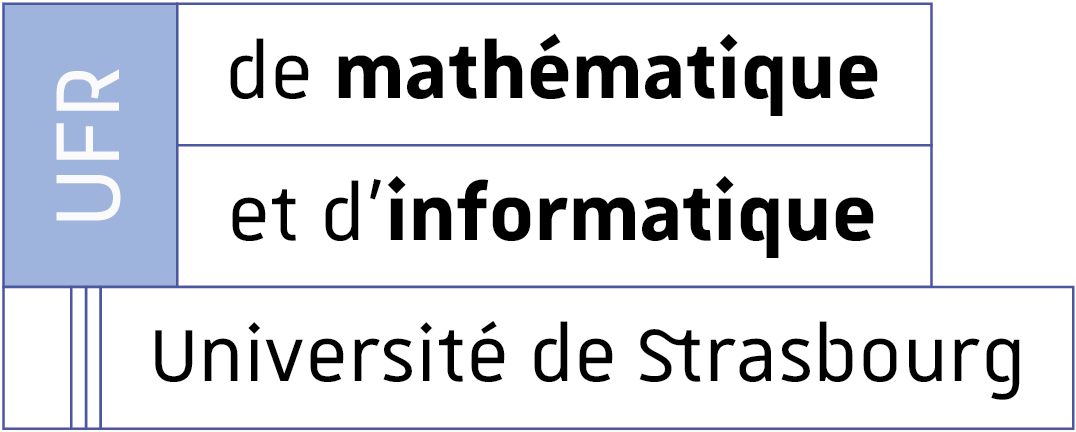
\includegraphics[width=7cm]{ufr.jpeg}};
		\end{tikzpicture}
		
		\begin{tikzpicture}[remember picture, overlay]
			\node[anchor=north east, inner sep=10pt] at (current page.north east) {
\includegraphics[width=7cm]{logo_E3S.PNG}};
		\end{tikzpicture}
		
		\vspace*{1cm}
		
		\begin{center}
			{\Large UNIVERSITE DE STRASBOURG} \par
			\vspace*{0.5cm}
			{\Large Master 1 Mathématiques et Applications} \par
			\vspace*{0.5cm}
			{\Large Parcours Statistique} \par
			\vspace*{3cm}
			{\Huge Rapport de stage au sein de l'Equipe de recherche E3S} \par
			\vspace*{0.5cm}
			{\Large Du 01 Avril 2024 au 30 Juin 2024} \par
			\vspace{1cm}
			{\Large \textbf{\textit{\underline{Thème}}} :} \par
			\vspace{1cm}
			\fbox{\parbox{12cm}{\centering \textcolor{black}{\Large Examen des conditions qui influencent les différences entre les sexes en matière d'engagement dans l'activité physique pendant les cours d'éducation physique, dans le cadre du contexte écologique}}} \par
			\vspace{0.5cm}
		\end{center}
		
		\vspace{1.5cm}
		{\Large \textbf{\textit{Stagiaire}} : Kossi Tonyi Wobubey ABOTSI} \par
		\vspace{0.5cm}
		{\Large \textbf{\textit{Tuteur référent}} : Christophe SCHNITZLER (Maître de Conférences à F3S, Université de Strasbourg)} \par
		\vspace{0.5cm}
		{\Large \textbf{\textit{Enseignant référent}} : Nicolas POULIN (Ingénieur de recherche au CeStatS, Université de Strasbourg)} \par
		
	\end{titlepage}
	
	
	% \thispagestyle{empty} % Supprime le numéro de page de la page de titre
	
	\newpage
	% Table des matière
	\renewcommand{\contentsname}{Table des matières} 
	\tableofcontents
	\newpage
	\section*{Préambule}
	\sectionmark{Préambule}
	\addcontentsline{toc}{section}{Préambule}
	Ce stage a eu lieu au sein de l'équipe de recherche "Sport et Sciences Sociales" (E3S - Équipe d'accueil n°1342), une unité de recherche en Sciences et Techniques des Activités Physiques et Sportives (STAPS) de l'Université de Strasbourg, reconnue par le ministère de l'Éducation nationale, de l'Enseignement supérieur et de la Recherche, et soumise à contractualisation. Le laboratoire E3S est situé au 4 rue René Descartes - 67084 Strasbourg Cedex.\\
	
	Il a été effectué sous la supervision de M. Christophe Schnitzler, avec le soutien de la doctorante Ornela Goldstein.\\
	
	Ce document a été entièrement rédigé en \LaTeX{} et tous les calculs ont été effectués à l'aide du logiciel \texttt{R} (version 4.3.3).
	
	
	

	\newpage
	\section*{Remerciement}
	\sectionmark{Remerciement}
	\addcontentsline{toc}{section}{Remerciement}
	Je tiens à remercier le laboratoire E3S et tout particulièrement mon tuteur de stage, M. Christophe SCHNITZLER, pour la confiance qu'il m'a accordée en me confiant des tâches décisives pour son projet. Il m'a accompagné et m'a accordé des entretiens lorsque j'en avais besoin. Je le remercie pour sa bienveillance à mon égard.\\
	
	Je remercie également la doctorante Ornela GOLDSTEIN, qui m'a accompagnée tout au long du projet et s'est rendue disponible pour moi durant tout le stage. Je la remercie pour ses conseils professionnels et techniques liés au domaine de l'éducation physique, ainsi que pour la patience dont elle a fait preuve.\\
	
	Je tiens à remercier M. Nicolas POULIN, ingénieur de recherche au CeStatS, Université de Strasbourg et M. Laurent GARDES, Professeur à l'Université de Strasbourg et responsable du Master de Statistique, pour leur aide précieuse pendant la recherche de stage.\\
	
	Je remercie tout le personnel du laboratoire E3S et toutes les personnes qui ont contribué à ce que ce stage se déroule dans les meilleures conditions, en particulier mes camarades stagiaires pour leurs remarques et apports lors de nos rencontres.

	% Contenu du rapport
	\newpage
\section*{Introduction}
\sectionmark{Introduction}
\addcontentsline{toc}{section}{Introduction}

L'Organisation Mondiale de la Santé (OMS) définit l'activité physique (AP) comme "tout mouvement corporel produit par les muscles squelettiques entraînant une dépense énergétique", englobant les activités réalisées durant les loisirs, le travail ou les déplacements.\\
Dans ce contexte, la baisse du niveau d'activité physique et l'augmentation de la sédentarité représentent des enjeux sanitaires et sociaux majeurs dans nos sociétés. Selon l'OMS, plus d'un quart de la population mondiale adulte n'est pas suffisamment active, et les niveaux de sédentarité sont deux fois plus élevés dans les pays à revenu élevé que dans les pays à faible revenu \cite{who2021}. La recherche met en avant des liens entre un niveau d’activité physique insuffisante et des risques accrus de maladies non transmissibles, de problèmes cardiaques, ainsi que des risques accrus d’obésité et de diabète de type 2 \cite{onaps2024campagne}. Aux problèmes sanitaires s’ajoutent des enjeux socio-économiques, avec des dépenses de santé estimées à 53,8 milliards de dollars et des pertes de productivité de 13,7 milliards liées à l’inactivité physique \cite{who2021}.\\
Les adolescents sont particulièrement touchés par ce manque d'activité physique, avec 81\% des adolescents ne remplissant pas les recommandations de l'OMS en termes d'activité \cite{who2021}.\\
Malgré des progrès significatifs dans la promotion de l'équité entre les sexes dans divers domaines, l'égalité réelle reste difficile à atteindre dans de nombreux aspects de la société \cite{UN_SDG_2020}, y compris en matière d'activité physique. Dans le contexte de l'éducation physique et sportive (EPS), cette disparité est visible dans les résultats d'évaluation, où les filles obtiennent des notes significativement inférieures à celles des garçons, un écart qui s'est accentué au fil du temps \cite{lentillon2005}.\\
Dans ce cadre, l'objectif de mon stage est d'examiner le niveau d'engagement physique des filles et des garçons lors d'une leçon d'EPS de 2 heures en mesurant leur MVPA\footnote{\textbf{MVPA (Moderate to Vigorous Physical Activity) ou en français, activité physique d'intensité modérée à vigoureuse, est un terme utilisé pour décrire des niveaux d'activité physique qui augmentent ou diminuent significativement la fréquence cardiaque. La mesure la plus courante de l'activité physique modérée à vigoureuse est le temps passé à effectuer ces activités. Par exemple, on pourrait mesurer combien de minutes par jour ou par semaine une personne passe en activité modéré à intense.}}, puis d'analyser cet écart en fonction de trois variables : la nature de l'activité (CA = champ d'apprentissage), la catégorie socioculturelle de l'établissement (catégorie d'IPS = indice de position sociale) et le milieu géographique (urbain ou rural).\\
Je présente dans ce document le travail réalisé au cours de mon stage. En premier lieu, je présente la théorie mathématique sous-jacente à mon travail (test de Student et ANOVA à deux facteurs avec plan non équilibré). Ensuite, je présente les statistiques descriptives sur les données disponibles et les résultats des analyses effectuées : test de Student et ANOVA à deux facteurs. Enfin, une partie annexe sur les codes \texttt{R} utilisés pour les calculs est brièvement exposée.

	\newpage
\section{Problématique et Contexte de l'étude}
La discipline de l'éducation physique et sportive (EPS) est également confrontée à des questions d'équité entre les sexes. Les recherches mettent en évidence des inégalités importantes : en moyenne, les filles obtiennent des résultats moins bons que les garçons lors des évaluations sommatives en EPS \cite{lentillon2005}. Par ailleurs, les interactions entre enseignants et élèves varient selon le sexe, avec une attention et des retours moins fréquents pour les filles comparativement aux garçons \cite{bonniotpaquien2009a}.\\
Les problèmes sanitaires et sociaux liés à l'inactivité physique soulignent la nécessité de se concentrer sur les populations les plus vulnérables. L'adolescence est une période particulièrement critique pour les filles en ce qui concerne leur relation avec l'activité physique. Ces enjeux sanitaires, conjugués aux questions d'équité entre les sexes, rendent l'engagement des filles dans l'activité physique particulièrement important. L'objectif de ce stage est d'examiner les différences d'engagement physique entre filles et garçons lors d'un cours d'EPS de 2 heures, en tenant compte de trois variables : la nature de l'activité (CA = champ d'apprentissage), la catégorie socioculturelle de l'établissement (catégorie d'IPS = indice de position sociale) et le milieu géographique.\\
Pour réaliser cette étude, nous avons inclus des collégiens de cycle 4 (de la 5ème à la 3ème), issus de classes ordinaires et ayant rendu les autorisations parentales, âgés de 11 à 15 ans. Ces élèves, provenant de collèges allant de très défavorisés à très favorisés et souhaitant participer à l’étude, ont rempli un premier questionnaire avant le début de l'étude afin de recueillir leurs données personnelles : âge, taille, poids, composition de la fratrie, pratique d’activité physique (AP) et autres informations socio-culturelles. Ensuite, les élèves ont été équipés d'accéléromètres (ActiGraph, modèle GT3X+) pour mesurer leur niveau de MVPA pendant un cours obligatoire d'EPS de 2 heures dans un champ d'apprentissage\footnote{\textbf{Champ d'apprentissage : 
		\begin{itemize}[label=--, leftmargin=*]
			\item CA1 : sports de performance (athlétisme, natation, cyclisme, ...)
			\item CA2 : sports de plein air et d'aventure (randonnée, alpinisme, surf, ...)
			\item CA3 : activité artistique (gymnastique rythmique, patinage artistique, ...)
			\item CA4 : sports d'opposition (sports de combat, tennis, ...)
	\end{itemize}}} spécifique. La collecte de données a été effectuée dans des collèges en Alsace et en Île-de-France, classés selon l’indice de position sociale (catégorie d'IPS) : écoles défavorisées (IPS < 89), écoles moyennes (90 <= IPS <= 114) et écoles favorisées (IPS > 115).\\
	Au total, 462 observations et 28 variables ont été recueillies.\\
	Pour atteindre l'objectif de l'étude, nous nous intéresserons à l'écart de MVPA par rapport à la moyenne de MVPA de chaque classe, afin d'examiner le niveau d'engagement entre les filles et les garçons en EPS. Ce choix est motivé par le fait que certaines classes présentent des durées d'activité différentes, des enseignants distincts et des infrastructures sportives variées, ce qui peut influencer le MVPA mesuré directement sur les participants. Ainsi, analyser le niveau d'engagement entre filles et garçons en fonction de l'écart de MVPA par rapport à la moyenne de chaque classe permet d'éliminer ces effets et facilite la comparaison.\\
	
	Voici un aperçu des premières lignes de mes données avec les colonnes utiles pour cette étude : 
	
	\begin{figure}[H]
		\centering
		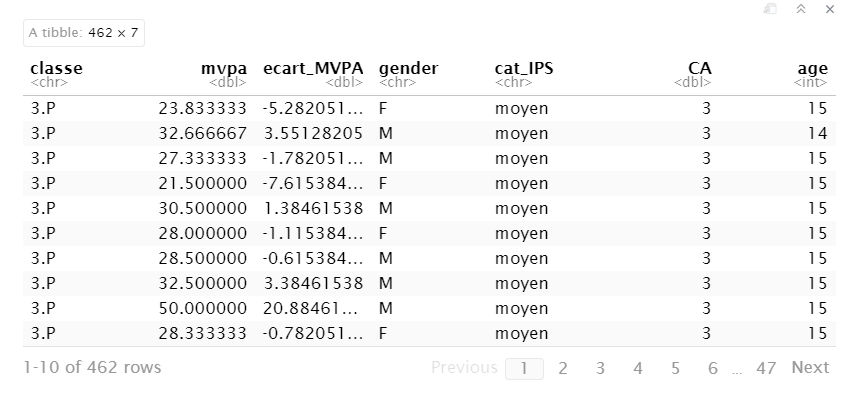
\includegraphics[width=\linewidth]{Extrai_donnée.PNG}
		\caption{Extraits des données}
		\label{fig:image1}
	\end{figure}


	
	
	\newpage
	\section{Présentation théorique}
	\subsection{Test de Student}
	Le test de Student est une méthode statistique utilisée pour comparer les moyennes d’une variable aléatoire quantitative
	dans différents groupes (variable qualitative) \cite{poulin2023}. Il est particulièrement utile pour comparer les moyennes de deux groupes. Au-delà de deux groupes, on utilise une ANOVA \cite{poulin2023}.
	
	\subsubsection{Hypothèses du test de Student et conditions d'application}
	Soit A et B deux échantillons sur lesquels on veut faire le test, avec des effectifs respectifs $n_A, n_B$.\\
	Soit Y la variable quantitative mesurée et $Y_A$, $Y_B$ les variables Y respectivement pour les groupes A et B.\\
	
	On pose : \\
	
	\noindent
	$\mu_A = \mathbb{E}[Y_A]$ et $\mu_B = \mathbb{E}[Y_B]$\\
	
	\noindent
	$\sigma_A^2 = Var[Y_A]$ et $\sigma_B^2 = Var[Y_B]$\\
	
	Ici on teste :
	\begin{equation*}
		H_0 : \mu_A = \mu_B \quad contre \quad H_1 : \mu_A \neq \mu_B
	\end{equation*}
	\textbf{Conditions d'application} \cite{poulin2023} : 
	\begin{itemize}[label=$\bullet$]
		\item Chaque échantillon est composé d'observations indépendantes.
		\item Les deux échantillons sont indépendants.
		\item $Y_A \sim \mathcal{N}(\mu_A,\sigma_A)$ et $Y_B \sim \mathcal{N}(\mu_B,\sigma_B)$ avec $\sigma_A$ et $\sigma_B$ inconnus.
		\item Égalité des variances dans les deux groupes $\sigma_A = \sigma_B$. Cette hypothèse peut être testée avec le test de Fisher-Snedecor.
	\end{itemize}
	
	\subsubsection{Statistique de décision}
	Après validation des conditions d'application, notons \( T \) la statistique de test.\\
	On a :
	\begin{equation}
		T = \frac{\overline{Y}_A - \overline{Y}_B}{S_p \times \sqrt{\frac{1}{n_A} + \frac{1}{n_B}}}\quad \text{où} \quad S_p = \sqrt{\frac{(n_A - 1)S_{Y_A}^2 + (n_B - 1)S_{Y_B}^2}{n_A + n_B - 2}}
	\end{equation}
	Avec \( S_{Y_A} = \sqrt{\frac{1}{n_A - 1}\sum_{i=1}^{n_A}(Y_{A,i} - \overline{Y}_A)^2} \) et \( S_{Y_B} = \sqrt{\frac{1}{n_B - 1}\sum_{i=1}^{n_B}(Y_{B,i} - \overline{Y}_B)^2} \) des estimateurs sans biais de \(\sigma_A\) et \(\sigma_B\), et \( S_p \) l'écart-type global de ces deux échantillons \cite{wikipedia_ttest}.\\
	
	\noindent
	Sous \( H_0 \), \( T \) suit une loi de Student à \( n_A + n_B - 2 \) degrés de liberté \cite{poulin2023}.
	
	\subsubsection{Taille d'effet}
	\begin{mdframed}[backgroundcolor=gray!20, hidealllines=true, innermargin=10pt, outermargin=10pt, skipabove=10pt, skipbelow=10pt, nobreak=true]
			La mesure de l'ampleur de l'effet la plus couramment utilisée pour un test de Student est le \textbf{d de Cohen} noté \textbf{"d"}.
		\begin{equation}
			d = \frac{\overline{Y}_A-\overline{Y}_B}{\hat{\sigma}} 
		\end{equation} 
		où $\hat{\sigma}$ est l'estimateur de l'écart type identique dans les deux groupes \cite{navarro2021}.\\
	\end{mdframed}
	
	\noindent
	\textit{\underline{Interprétation du d de Cohen}} : \\
	
	la statistique d est interprétée comme une description de la différence entre les moyennes comme étant le nombre d'écarts-types qui sépare ces moyennes \cite{navarro2021}.
	\begin{itemize}[label=$\bullet$]
		\item $d \approx 0.2$ : petit effet
		\item $d \approx 0.5$ : effet moyen
		\item $d \approx 0.8$ : grand effet
	\end{itemize}
	
	\subsection{Analyse de variance à 2 facteurs}
	L'analyse de variance (ANOVA) est une méthode permettant de modéliser la relation entre une variable quantitative et une ou plusieurs variables qualitatives. Lorsqu'il y a une seule variable explicative, on parle d'analyse de variance à un facteur. Cette méthode permet de comparer k (k$>$2) moyennes et peut donc être vue comme une extension du test de comparaison de moyennes (Test de Student).
	
	Ici, nous allons nous intéresser au cas de deux variables explicatives qualitatives, donc à l'analyse de variance à deux facteurs, que l'on peut toutefois généraliser à un nombre quelconque de variables explicatives.
	
	\subsubsection{Modèle d'analyse de variance (ANOVA à deux facteurs)}
	\begin{mdframed}[backgroundcolor=gray!20, hidealllines=true, innermargin=10pt, outermargin=10pt, skipabove=10pt, skipbelow=10pt, nobreak=true]
			Notons A et B deux variables explicatives qualitatives, et Y une variable explicative quantitative. Soit I le nombre de modalités de A et J celui de la variable B.
		Le modèle s'écrit classiquement :
		\begin{equation*}
			Y_{ijk} = \mu + \alpha_i + \beta_j + \gamma_{ij} + \epsilon_{ijk}, \quad i = 1, \ldots, I; j = 1, \ldots, J;  \epsilon_{ijk} \overset{\text{i.i.d}}{\sim} \mathcal{N}(0,\sigma^2)
		\end{equation*}
		avec un effet moyen général $\mu$, $\alpha_i$ représente l'effet principal du facteur A, $\beta_j$ représente l'effet principal du facteur B, un terme d'interaction $\gamma_{ij}$ et un résidu $\epsilon_{ijk}$ avec $k$ l'indice de répétition pour le couple $(i,j)$ \cite{daudin}.
	\end{mdframed}
	Le modèle n'est pas identifiable car pour un $(1+I+J+IJ)$-uplet $(\mu,\alpha_1,...,\alpha_I,\beta_1,...,\beta_J,\gamma_{11},$\\$..., \gamma_{ij},...,\gamma_{IJ})^T$ et $a \in \mathbb{R}$, le $(1+I+J+IJ)$-uplet $(\mu-a,\alpha_1+\frac{a}{3},...,\alpha_I+\frac{a}{3},\beta_1+\frac{a}{3},...,\beta_J+\frac{a}{3},\gamma_{11}+\frac{a}{3},...,\gamma_{ij}+\frac{a}{3},...,\gamma_{IJ}+\frac{a}{3})^T$ correspond au même modèle. On a donc besoin de contraintes sur les paramètres.\\
	
	Les contraintes classiques sont \cite{cornillon2022regression}: 
	\begin{itemize}[label=--, leftmargin=*]
		\item Contrainte d'analyse par cellule
		\begin{equation*}
			\mu=0,\quad\quad \forall i \quad  \alpha_i=0, \quad\quad \forall  j  \quad \beta_j=0.
		\end{equation*}
		\item Contrainte avec cellule de référence
		\begin{equation*}
			\alpha_1=0,\quad\quad \beta_1=0,\quad\quad \forall i\quad \gamma_{i1}=0,\quad\quad \forall j \quad \gamma_{1j}=0
		\end{equation*}
		\item Contrainte de somme
		\begin{equation*}
			\sum_{i}\alpha_i=0,\quad\quad\sum_{j}\beta_j=0,\quad\quad\forall i \quad \sum_{j}\gamma_{ij}=0,\quad\quad\forall j \quad\sum_{i}\gamma_{ij}=0
		\end{equation*}
	\end{itemize}
	
	\subsubsection{Conditions d'application}
	Un modèle d'ANOVA à deux facteurs doit satisfaire trois conditions \cite{maistre2023} :
	\begin{itemize}[label=$\bullet$]
		\item Indépendance des observations (ou des résidus).
		\item Égalité des variances des résidus du modèle (homoscédasticité).
		\item Normalité des résidus du modèle.
	\end{itemize}

	
	
	\subsubsection{Test de l'interaction et de significativité des effets de facteur}
	Pour tester l'effet d'un facteur, il est naturel de tester la nullité des paramètres associés à chaque niveau de ce facteur. Cette approche est insuffisante pour définir correctement l'hypothèse nulle testée, il faut préciser les hypothèses portant sur les autres facteurs et interactions. Si le plan est équilibré, quelles que soient les hypothèses portant sur les autres variables, le test de significativité de facteur reste identique pour le même facteur \cite{daudin}. Cependant, dans le cas de plan déséquilibré, ce test peut parfois différer en fonction des hypothèses portant sur les autres facteurs et interactions. On utilise donc la notion de réduction, définie ci-dessous, qui permet de bien spécifier le rôle des autres facteurs et interactions.\\
	
	\begin{mdframed} [backgroundcolor=gray!20, hidealllines=true, innermargin=10pt, outermargin=10pt, skipabove=10pt, skipbelow=10pt, nobreak=true]
		\textbf{Définition :}\\
			 Soit un modèle contenant les effets $(a_1,\ldots,a_l)$ des facteurs $(X_1, X_2, \ldots, X_l)$. On appelle réduction associée à l'introduction de $a_{q_1}, \ldots, a_{q_d}$ dans un modèle contenant les effets $a_{i_1}, \ldots, a_{i_m}$, notée $R(a_{q_1}, \ldots, a_{q_d}|\mu,a_{i_1}, \ldots, a_{i_m})$ la norme suivante : 
		
		\begin{equation}
			R(a_{q_1}, \ldots, a_{q_d}|\mu,a_{i_1}, \ldots, a_{i_m}) = SCE_{i_1,i_2,\ldots,i_m,q_1,q_2,\ldots,q_d} - SCE_{i_1,i_2,\ldots,i_m},
		\end{equation}
		
		avec $SCE_{i_1,i_2}$ la somme des carrés expliquée par le modèle associée aux facteurs $X_{i_1}$, $X_{i_2}$ \cite{daudin}.
	\end{mdframed}
	
	Soit $\alpha, \beta$ et $\gamma$ les effets respectifs des deux facteurs principaux A, B et de l'interaction $A*B$ dans le modèle.
	
	La variabilité de Y se décompose en la somme de deux termes \cite{maistre2023}: 
	\begin{equation}
		SCT = SCE + SCR
	\end{equation}
	
	On a donc 
	\begin{equation}
		R(\alpha|\mu,\beta,\gamma) = SCE_1 - SCE_2,
	\end{equation}
	où $SCE_1$ et $SCE_2$ sont respectivement la somme des carrés expliquée des modèles\\
	
	\noindent
	$(M_1) : Y_{ijk} = \mu + \alpha_i + \beta_j + \gamma_{ij} + \epsilon_{ijk}$\\
	$(M_2) : Y_{ijk} = \mu + \beta_j + \gamma_{ij} + \epsilon_{ijk}$\\
	pour tout $i = 1,\ldots,I$, $j = 1,\ldots,J$, $k = 1,\ldots,K$ \cite{daudin}.\\
	
	Un test de l'effet d'un facteur est associé à une réduction donnée. Considérons la réduction $R(\alpha|\mu,\beta,\gamma)$, les hypothèses associées s'écrivent : 
	\begin{itemize}[label=--, leftmargin=*]
		\item $H_0$ : Il n'y a pas de différence significative entre le modèle ne contenant pas l'effet du facteur A et le modèle complet.
		\item $H_1$ : Il y a une différence significative entre le modèle ne contenant pas l'effet du facteur A et le modèle complet.
	\end{itemize}
	La statistique de test est donnée par : 
	\begin{equation}
		F = \frac{\frac{R(\alpha|\mu,\beta,\gamma)}{I-1}}{\frac{\text{SCR}}{n-IJ}},
	\end{equation}
	où 
	\begin{itemize}[label=--, leftmargin=*]
		\item $I-1$ est le nombre de contraintes dans l'hypothèse nulle.
		\item $IJ$ est le nombre de paramètres de notre modèle.
	\end{itemize}
	Sous $H_0$, $F \sim \mathcal{F}(I-1, n-IJ)$ \cite{daudin}. \\
	
	\noindent
	\textbf{Quelques réductions classiques :} \\
	Parmi les plus classiques, on trouve les réductions de type I, type II et type III \cite{daudin}.
	
	\begin{enumerate}[label=\textbf{\alph*})]
		\item \textbf{Somme des carrés de type I}\\
		La réduction de type I provient de la décomposition de la somme des carrés expliquée par le modèle en réductions successives. Elle consiste à ajouter au modèle un des termes à la fois. Dans le modèle $M_1$ ci-dessus \cite{navarro2021},
		\begin{equation}
			SCE_1 = R(\alpha,\beta,\gamma|\mu) = R(\alpha|\mu) + R(\beta|\alpha,\mu) + R(\gamma|\alpha,\beta,\mu)
		\end{equation}
		La table \ref{ref:analyse_var_1} présente la table d'analyse de variance pour le modèle $M_1$.
		\begin{table}[H]
			\centering
			\caption{Table d'analyse de la variance des réductions de type I du modèle $M_1$ \cite{daudin}.}
			\begin{tabular}{|c|c|c|c|p{6cm}|}
				\hline
				\textbf{Effet} & \textbf{Réduction type I} & \textbf{DDL} & \textbf{F} & \textbf{Question} \\
				\hline
				$\alpha$ & $R(\alpha|\mu)$ & $I-1$ & \LARGE{$\frac{\frac{R(\alpha|\mu)}{I-1}}{\frac{\text{SCR}}{n-IJ}}$} & Est-il pertinent d'ajouter l'effet du facteur A à un modèle ne contenant que la constante ? \\
				\hline
				$\beta$ & $R(\beta|\mu, \alpha)$ & $J-1$ & \LARGE{$\frac{\frac{R(\beta|\mu, \alpha)}{J-1}}{\frac{\text{SCR}}{n-IJ}}$} & Est-il pertinent d'ajouter l'effet du facteur B à un modèle contenant la constante et l'effet du facteur A ? \\
				\hline
				$\gamma$ & $R(\gamma|\mu, \alpha, \beta)$ & $(I-1) \times (J-1)$ & \LARGE{$\frac{\frac{R(\gamma|\mu, \alpha, \beta)}{(I-1) \times (J-1)}}{\frac{\text{SCR}}{n-IJ}}$} & Est-il pertinent d'ajouter l'effet d'interaction entre les deux facteurs à un modèle contenant la constante et les effets des deux facteurs ? \\
				\hline
			\end{tabular}
		\label{ref:analyse_var_1}
		\end{table}
		
		\item \textbf{Somme des carrés de type II}\\
		Dans la réduction de type I, l'ordre d'introduction des facteurs dans le modèle leur confère un rôle différent ce qui ne représente aucun intérêt lorsque l'ordre n'est pas important pour notre sujet d'étude. L'idée des types II dans le cadre d'une ANOVA à deux facteurs, consiste à considérer la réduction portée par un facteur ou interaction conditionnellement aux autres facteurs (principaux) \cite{navarro2021}. Donc l'ordre n'est plus important mais aussi il prend en compte le principe qu'on ne peut pas supprimer l'effet d'un facteur principal du modèle sachant qu'il y a effet de l'interaction.
		La table \ref{ref:analyse_var_2} présente la table d'analyse de variance pour le modèle $M_1$.
		\begin{table}[H]
			\centering
			\caption{Table d'analyse de la variance des réductions de type II du modèle $M_1$ \cite{daudin}.}
			\begin{tabular}{|c|c|c|c|p{6cm}|}
				\hline
				\textbf{Effet} & \textbf{Réduction type II} & \textbf{DDL} & \textbf{F} & \textbf{Question} \\
				\hline
				$\alpha$ & $R(\alpha|\beta, \mu)$ & $I-1$ & \LARGE{$\frac{\frac{R(\alpha|\beta, \mu)}{I-1}}{\frac{\text{SCR}}{n - IJ}}$} & Est-il pertinent d'ajouter l'effet du facteur A à un modèle contenant la constante et l'effet du facteur B ? \\
				\hline
				$\beta$ & $R(\beta|\mu, \alpha)$ & $J-1$ & \LARGE{$\frac{\frac{R(\beta|\mu, \alpha)}{J-1}}{\frac{\text{SCR}}{n - IJ}}$} & Est-il pertinent d'ajouter l'effet du facteur B à un modèle contenant la constante et l'effet du facteur A ? \\
				\hline
				$\gamma$ & $R(\gamma|\mu, \alpha, \beta)$ & $(I-1) \times (J-1)$ & \LARGE{$\frac{\frac{R(\gamma|\mu, \alpha, \beta)}{(I-1) \times (J-1)}}{\frac{\text{SCR}}{n - IJ}}$} & Est-il pertinent d'ajouter l'effet de l'interaction entre les deux facteurs à un modèle contenant la constante et les effets des deux facteurs ? \\
				\hline
			\end{tabular}
		\label{ref:analyse_var_2}
		\end{table}
		
		\item \textbf{Somme des carrés de type III}\\
		La réduction de type III consiste à considérer la réduction portée par un facteur ou interaction conditionnellement aux autres facteurs ou à l'interaction \cite{navarro2021}.
		La table \ref{ref:analyse_var_3} présente la table d'analyse de variance pour le modèle $M_1$
		\begin{table}[H]
			\centering
			\caption{Table d'analyse de la variance des réductions de type III du modèle $M_1$.}
			\begin{tabular}{|c|c|c|c|p{6cm}|}
				\hline
				\textbf{Effet} & \textbf{Réduction type III} & \textbf{DDL} & \textbf{F} & \textbf{Question} \\
				\hline
				$\alpha$ & $R(\alpha|\beta, \mu, \gamma)$ & $I-1$ & \LARGE{$\frac{\frac{R(\alpha|\beta, \mu, \gamma)}{I-1}}{\frac{\text{SCR}}{n-IJ}}$} & Est-il pertinent d'ajouter l'effet du facteur A à un modèle contenant la constante, l'effet du facteur B et l'interaction ? \\
				\hline
				$\beta$ & $R(\beta|\mu, \alpha, \gamma)$ & $J-1$ & \LARGE{$\frac{\frac{R(\beta|\mu, \alpha, \gamma)}{J-1}}{\frac{\text{SCR}}{n - IJ}}$} & Est-il pertinent d'ajouter l'effet du facteur B à un modèle contenant la constante, l'effet du facteur A et l'interaction ? \\
				\hline
				$\gamma$ & $R(\gamma|\mu, \alpha, \beta)$ & $(I-1) \times (J-1)$ & \LARGE{$\frac{\frac{R(\gamma|\mu, \alpha, \beta)}{(I-1) \times (J-1)}}{\frac{\text{SCR}}{n - IJ}}$} & Est-il pertinent d'ajouter l'effet de l'interaction entre les deux facteurs à un modèle contenant la constante et les effets des deux facteurs ? \\
				\hline
			\end{tabular}
			\label{ref:analyse_var_3}
		\end{table}
	
	\end{enumerate}
	
	\textbf{NB}: l'ANOVA de type II sera préférée à celle de type III dans toute la suite dans le cas d'un plan déséquilibré.
	
	\subsubsection{Test de comparaison multiple}
	Si aucun des facteurs ni l'interaction n'est significatif, l'étude sera conclue. Dans le cas où au moins l'un des facteurs A ou B ou l'interaction est significatif, il pourrait être intéressant de comparer les moyennes (de population) entre les différents groupes afin de voir quels groupes sont différents des autres.
	Dans le cas où par exemple l'interaction est significative, les tests auront par exemple les hypothèses : 
	\begin{itemize}[label=--, leftmargin=*]
		\item $H_0 : \theta_{i_1j_1} = \theta_{i_2j_2}$
		\item $H_1 : \theta_{i_1j_1} \neq \theta_{i_2j_2}$
	\end{itemize}
	où $\theta_{i_1j_1}$ et $\theta_{i_2j_2}$ sont les moyennes dans chaque groupe différent et $i_1,i_2\in{1,...,I}$ ; $j_1,j_2\in{1,...,J}$.
	
	On veut comparer tous les groupes deux à deux. En comparant m groupes, on effectue $\frac{m(m-1)}{2}$ comparaisons à un niveau $\alpha$. Ce qui nous expose plus au risque de commettre une erreur de type I (accepter à tort $H_1$ à un niveau $\alpha$). Donc pour y remédier nous allons utiliser la méthode de Tukey pour un plan équilibré et Tukey-Kramer pour un plan complet \cite{maistre2023}.
	
	\begin{mdframed}[backgroundcolor=gray!20, hidealllines=true, innermargin=10pt, outermargin=10pt, skipabove=10pt, skipbelow=10pt, nobreak=true]
		\textbf{Méthode de Tukey(-Kramer) : }
		pour les tests de comparaison des m moyennes deux à deux, l'intervalle de confiance de Tukey(-Kramer) \cite{maistre2023} de niveau 1-$\alpha$ (Dans notre cas d'étude 95\%) pour $\theta_{i_1j_1} - \theta_{i_2j_2}$ est : 
		\begin{equation}
			\left [\bar{Y}_{i_1j_1}-\bar{Y}_{i_2j_2} \pm r^{(m,n-m)}_{(1-\alpha)}\sqrt{\frac{\hat{\sigma}^2}{2}\times\left(\frac{1}{n_{i_1j_1}}+\frac{1}{n_{i_2j_2}}\right)}\right]
		\end{equation}
		où $r^{(m,n-m)}_{(1-\alpha)}$ est le quantile d'ordre 1-$\alpha$ d'une loi spécifique à ce problème, la Studentized range distribution.\\
		On conservera $H_0$ pour les intervalles contenant 0.
	\end{mdframed}

	Il y a d'autres méthodes de correction qui ne seront pas abordées dans ce travail telles que : méthode de Scheffé, méthode de Holm-Bonferroni, correction de Bonferroni, etc.
	
	\subsubsection{Taille d'effet}
	\begin{mdframed}[backgroundcolor=gray!20, hidealllines=true, innermargin=10pt, outermargin=10pt, skipabove=10pt, skipbelow=10pt, nobreak=true]
		La taille d'effet dans un modèle d'analyse de variance est une mesure qui permet d'évaluer l'ampleur de la différence entre les groupes due à un effet.
		Pour le calcul de la taille d'effet, nous pouvons utiliser $\omega^2$ (omega-squared) comme moyen de mesure.
		$\omega^2$ est défini de la manière suivante \cite{wikipediaEffectSize} : 
		\begin{equation}
			\omega^2 = \frac{SCE_{facteur} - (k-1)\cdot MS_{erreur}}{SCT + MS_{erreur}} \quad \text{avec} \quad MS_{erreur} = \frac{SCR}{N-k}
		\end{equation}    
		où : 
		\begin{itemize}[label=--, leftmargin=*]
			\item $SCE_{facteur}$ est la somme des carrés expliquée par le facteur en question
			\item $SCT$ est la somme des carrés totale
			\item $SCR$ est la somme des carrés résiduels
			\item $k$ est le nombre de modalités du facteur
			\item $N$ est le nombre total d'observations
			\item $MS_{erreur}$ est la moyenne des carrés des erreurs au sein des groupes 
		\end{itemize}
	\end{mdframed}
	
	\noindent
	\textit{\underline{Interprétation}}  \\
	
	Il s'agit de la proportion de la variabilité de la variable dépendante qui peut être expliquée par le facteur en question. Une valeur de $\omega^2 = 0$ signifie qu'il n'y a aucune relation entre les deux, alors qu'une valeur de $\omega^2 = 1$ signifie que la relation est parfaite \cite{navarro2021}. 
	\begin{itemize}[label=--, leftmargin=*]
		\item Petite taille d'effet $\omega^2 \approx 0.01$
		\item Taille d'effet moyenne $\omega^2 \approx 0.06$
		\item Grande taille d'effet $\omega^2 \approx 0.14$
	\end{itemize}    
	
\newpage

\section{Résultats et Discussion}
\subsection{Analyse descriptive}
La première partie de mon stage consiste à effectuer une analyse descriptive des données après les avoir nettoyées. Les statistiques descriptives sont présentées dans le tableau \ref{tab:descriptive_stats}. Au total, nous avons eu 462 participants dans notre étude, dont 220 filles et 242 garçons. Les participants avaient en moyenne 13,65 ans. Parmi eux, 47,61\% sont des filles et 52,39\% sont des garçons. En termes de champs d'apprentissage, 12,13\% sont dans le champ 1, 26,15\% dans le champ 2, 10,24\% dans le champ 3 et environ 51,48\% dans le champ 4. En ce qui concerne les catégories d'IPS, 31\% sont dans la catégorie basse, 22,37\% dans la catégorie moyenne et 46,63\% dans la catégorie haute. Pour les zones géographiques, 64,15\% sont en zones urbaines et 35,85\% en zones rurales. La moyenne de MVPA pendant 2 heures pour les participants est de 35,14 minutes, avec 31,4 minutes pour les filles et 38,5 minutes pour les garçons. Les détails sur les catégories socio-professionnelles des parents sont présentés dans le tableau \ref{tab:descriptive_stats}, ainsi que le nombre de participants dont les parents occupent l'une des professions listées. Le tableau \ref{tab:descriptive_stats} montre également la proportion de filles et de garçons dans différents champs d'apprentissage, catégories d'IPS et zones géographiques. En général, les proportions de filles et de garçons selon les différentes variables sont similaires, sauf pour certaines modalités de ces variables.\\

\begin{table}[H]
	\centering
	\caption{Statistiques descriptives des participants}
	\begin{tabular}{lrrr}
		\toprule
		\textbf{Variables} & \textbf{Total} & \textbf{Filles} & \textbf{Garçons} \\
		\midrule
		\textbf{Participants} & \textbf{(n = 462)} & \textbf{(n = 220)} & \textbf{(n = 242)} \\
		Participants (\%) & 100\% & 47.61\% & 52.39\%\\
		Âge moyen & 13.65 & 13.66 & 13.65 \\
		\midrule
		\textbf{MVPA}\\
		\textbf{moyenne} & 35.14 & 31.4 & 38.5\\
		\textbf{médiane} & 34.83 & 31 & 37.67\\
		\textbf{écart-type} & 15.79 &  15.23& 15.57 \\
		\textbf{maximum} & 77.16 & 63.5 & 77.17 \\
		\textbf{minimum} &1.333 & 1.33 & 6\\
		\midrule
		\textbf{Catégories socio-professionnelles des parents (nombre)} \\
		Agriculteurs & 10 & 7 & 3 \\
		Artisans, commerçants, chefs d'entreprise & 106 & 59 & 47 \\
		Autres inactifs & 82 & 32 & 50 \\
		Cadres et professions intellectuelles supérieures & 99 & 52 & 47 \\
		Employés & 213 & 90 & 123 \\
		Ouvriers & 66 & 28 & 38 \\
		Professions intermédiaires & 116 & 59 & 57 \\
		Retraités & 7 & 4 & 3 \\
		NA & 43 & 23 & 20 \\
		\midrule
		\textbf{Champs d'apprentissage} \\
		Champ 1 (sports de performance) & 12.13\% & 5.12\% & 7.01\% \\
		Champ 2 (sports de plein air) & 26.15\% & 13.75\% & 12.40\% \\
		Champ 3 (activités artistiques) & 10.24\% & 4.31\% & 5.93\% \\
		Champ 4 (activités d'opposition) & 52.48\% & 24.53\% & 26.95\% \\
		\midrule
		\textbf{Catégories socioculturelles} \\
		Haute & 46.63\% & 16.17\% & 14.83\% \\
		Basse & 22.37\% & 11.86\% & 10.51\% \\
		Moyenne & 31\% & 19.68\% & 26.95\% \\
		\midrule
		\textbf{Zone géographique} \\
		Rurale & 35.85\% & 17.79\% & 18.06\% \\
		Urbaine & 64.15\% & 29.92\% & 34.23\% \\
		\bottomrule
	\end{tabular}
	\label{tab:descriptive_stats}
\end{table}

\subsection{Modèles d'ANOVA}
Tous les tests statistiques réalisés dans cette partie ont un seuil de significativité fixé à 5\%.

\subsubsection{Examen de l'écart de MVPA entre Filles et Garçons}
L'objectif ici est de déterminer si l'étude produit des résultats similaires à ceux des travaux antérieurs. Nous souhaitons examiner l'effet du genre sur le niveau d'engagement physique. La variable qualitative considérée est le genre (F pour les filles et M pour les garçons), et la variable quantitative est l'écart de MVPA par rapport à la moyenne de chaque classe. Dans toute la suite du document, \texttt{ecart\_MVPA} fera référence à l'écart de MVPA par rapport à la moyenne de MVPA de chaque classe. Soit $Y_F$ et $Y_M$ les variables quantitatives correspondant à \texttt{ecart\_MVPA} pour les groupes de filles et de garçons, respectivement.\\


\noindent
\begin{enumerate}[label=\textbf{\alph*})]
	\item \textbf{Hypothèses et Test à utiliser}  \\
	
	Pour déterminer s'il y a un effet du genre sur le niveau d'engement physique, nous allons comparer les moyennes de \texttt{ecart\_MVPA} des deux groupes (Fille et Garçon). Nous voulons tester les hypothèses suivantes : 
	\begin{equation*}
		H_0 : \mu_F = \mu_G \quad contre \quad H_1 : \mu_F \neq \mu_G
	\end{equation*}
	Avec $\mu_F = \mathbb{E}[Y_F]$ et $\mu_G = \mathbb{E}[Y_G]$.\\
	
	 La table \ref{tab:desc_stats_genre} contient les statistiques descriptives pour les deux groupes.
	\begin{table}[H]
		\centering
		\caption{Statistiques descriptives par genre}
		\begin{tabular}{lcccccc}
			\toprule
			\textbf{gender} & \textbf{Effectif} & \textbf{Moyenne\_ecart\_MVPA} & \textbf{Ecart\_type} & \textbf{min} & \textbf{max} \\
			\midrule
			F & \multicolumn{1}{c}{220} & \multicolumn{1}{c}{-2.919044} & \multicolumn{1}{c}{8.524157} & \multicolumn{1}{c}{-35.94253} & \multicolumn{1}{c}{14.22414} \\
			M & \multicolumn{1}{c}{242} & \multicolumn{1}{c}{2.653677} & \multicolumn{1}{c}{8.502965} & \multicolumn{1}{c}{-38.77586} & \multicolumn{1}{c}{23.41667} \\
			\bottomrule
		\end{tabular}
		\label{tab:desc_stats_genre}
	\end{table}
	
	Pour tester $H_0$ contre $H_1$, nous allons utiliser le \textbf{test de Student}. Vérifions donc les conditions d'application.\\
	
\noindent
\item \textbf{Vérifications des conditions d'application} \\

\noindent
\textbf{Indépendance} : chaque échantillon est composé d'observations indépendantes, et les deux échantillons eux-mêmes sont indépendants. La liaison potentielle due à l'appartenance à une même classe ou école est éliminée en utilisant l'écart à la moyenne du MVPA pour chaque classe, plutôt que le MVPA brut.\\

\noindent
\textbf{Normalité des deux groupes} : nous voulons vérifier si les variables aléatoires $Y_F$ (pour les filles) et $Y_G$ (pour les garçons) suivent une distribution normale. La figure \ref{fig:QQplot_1} présente les Q-Q plots des deux groupes. On observe que l'hypothèse de normalité est raisonnable dans les deux groupes, car les points sur les graphiques sont globalement alignés sur les deux lignes diagonales, à l'exception des queues des distributions. De plus, avec des tailles d'échantillon relativement grandes (220 pour les filles et 242 pour les garçons), le test de Student est relativement robuste à la non-normalité \cite{poulin2023}.

\begin{figure}[H]
	\centering
	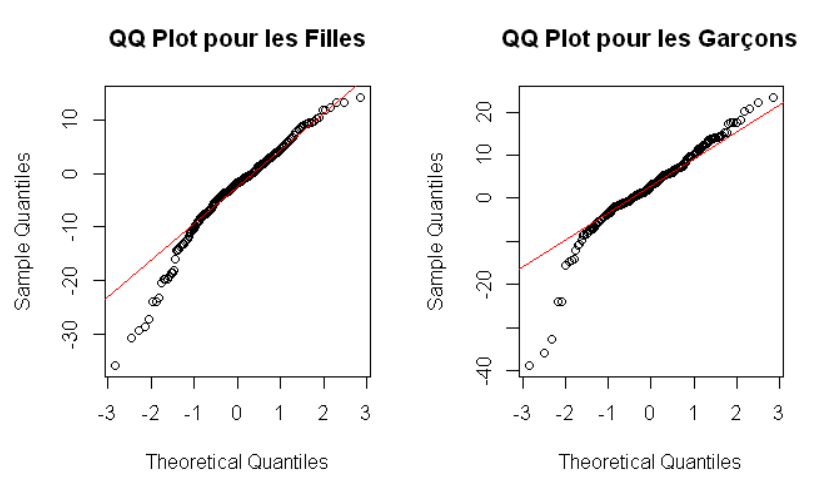
\includegraphics[width=\linewidth]{QQ_plot_deux_goupe.PNG}
	\caption{Q-Q plot des deux groupes : Filles et Garçons}
	\label{fig:QQplot_1}
\end{figure}

\noindent
\textbf{Égalité des variances (inconnues) des deux groupes} : pour tester l'égalité des variances théoriques (qui sont inconnues) entre les deux groupes, nous utilisons le test de \textbf{Fisher-Snedecor}. Nous testons les hypothèses suivantes :
\begin{equation*}
	H_0 : \sigma_F = \sigma_G \quad \text{contre} \quad H_1 : \sigma_F \neq \sigma_G
\end{equation*}
où $\sigma_F$ et $\sigma_G$ représentent respectivement les écarts types théoriques des groupes Filles et Garçons.\\

\noindent
\textit{\underline{Condition d'application et test de Fisher-Snedecor}} \\

Les hypothèses d'indépendance et de normalité ayant été vérifiées précédemment, nous pouvons procéder au test de Fisher-Snedecor.\\
La statistique de test observée est $F = \frac{S_{Y_F}^2}{S_{Y_G}^2} = 1.005$. Sous $H_0$, $F$ suit une loi de Fisher avec $n_F - 1 = 219$ et $n_G - 1 = 241$ degrés de liberté. La p-valeur obtenue est de 0.9683, ce qui est supérieur à 5\%. Nous ne pouvons donc pas rejeter $H_0$, ce qui signifie que nous n'avons pas de preuve suffisante pour affirmer que les variances des deux groupes sont différentes.\\

	
	\textbf{\textit{Toutes les conditions d'application du test de Student étant respectées, nous pouvons donc réaliser ce test.}} \\
	
	Nous observons une statistique de test $T = \frac{\overline{Y_F} - \overline{Y_G}}{\sqrt{\frac{S_{Y_F}^2}{n_F} + \frac{S_{Y_G}^2}{n_G}}} = -7.0272$. Sous $H_0$, T suit une loi de Student avec $n_F + n_G - 2 = 460$ degrés de liberté. La p-valeur obtenue est $7.642 \times 10^{-12}$, qui est inférieure au seuil de 5\%. Nous ne pouvons donc pas accepter $H_0$. Ainsi, la moyenne de \texttt{ecart\_MVPA} des garçons est significativement supérieure à celle des filles (T < 0). Donc les garçons s'engagent plus que les filles en EPS\\

	
	\noindent
	\item \textbf{Taille d'effet (d de Cohen)} \\
	
	D'après le test de Student, les garçons ont en moyenne un \texttt{ecart\_MVPA} significativement supérieur à celui des filles. Ici, nous souhaitons mesurer l'ampleur de cette différence à l'aide du \(d\) de Cohen. \\
	La table \ref{effect_size_1} présente le calcul de la taille d'effet (Cohen's \(d\)). 
	\begin{table}[H]
		\centering
		\caption{Estimation de \(d\) de Cohen et intervalle de confiance à 95\%}
		\begin{tabular}{ccc}
			\toprule
			Paramètre & \(d\) estimé & IC à 95\% \\
			\midrule
			Cohen's \(d\) & 0.65 & [0.47, 0.84] \\
			\bottomrule
		\end{tabular}
		\label{effect_size_1}
	\end{table}
	
	La valeur de \(d\) de Cohen est de 0.65. Ainsi, la moyenne de \texttt{ecart\_MVPA} des garçons est 0.65 écart-type plus élevée que la moyenne de \texttt{ecart\_MVPA} des filles, ce qui correspond à un effet de taille modéré. Cette différence est donc suffisamment importante pour être considérée dans la pratique.
	
\end{enumerate}

\subsubsection{Examen de l'écart de MVPA entre Filles et Garçons selon le CA}
	Nous souhaitons étudier l'effet du genre et du champ d'apprentissage sur le niveau d'engagement physique en EPS. Pour ce faire, nous utilisons un modèle d'ANOVA à deux facteurs (genre et champ d'apprentissage) avec comme variable dépendante l'écart de MVPA par rapport à la moyenne de MVPA de chaque classe. Pour les contraintes du modèle, nous appliquons la contrainte de somme nulle. Le modèle s'écrit :
	\begin{equation}
		Y_{ijk} = \mu + \alpha_i + \beta_j + \gamma_{ij} + \epsilon_{ijk}, \quad \epsilon_{ijk} \overset{\text{i.i.d}}{\sim} \mathcal{N}(0, \sigma^2) \tag{M1}
	\end{equation}
	\noindent
	où $i = 1, \ldots, 2$, $j = 1, \ldots, 4$. Ici, $\mu$ est l'effet moyen général, $\alpha_i$ représente l'effet principal du genre, $\beta_j$ représente l'effet principal du champ d'apprentissage, $\gamma_{ij}$ est le terme d'interaction, et $\epsilon_{ijk}$ sont les résidus avec $k$ l'indice de répétition pour le couple $(i, j)$. La variance résiduelle est notée $\sigma^2$.\\

\begin{enumerate}[label=\textbf{\alph*})]
	\item \textbf{Plan et visualisation des données}\\
	
	La table \ref{tab:ca_gender} présente les effectifs des différents CA par genre. On observe que le nombre d’observations varie selon le croisement des modalités de CA et genre. Par conséquent, nos données sont déséquilibrées. Dans ce contexte, nous utilisons l'ANOVA de type II car l'ordre des facteurs n'a pas d'importance dans cette étude.\\
	
	\begin{table}[H]
		\centering
		\caption{Effectifs des CA par genre}
		\begin{tabular}{ccccc}
			\toprule
			& CA 1 & CA 2 & CA 3 & CA 4 \\ 
			\midrule
			F & 20 & 53 & 49 & 98 \\ 
			M & 26 & 51 & 54 & 111 \\ 
			\bottomrule
		\end{tabular}
		\label{tab:ca_gender}
	\end{table}
	
	La table \ref{tab:desc_stats_CA} présente les statistiques descriptives pour les différents groupes.\\
	
	\begin{table}[H]
		\centering
		\caption{Statistiques descriptives par genre et CA}
		\begin{tabular}{ccrcccc}
			\toprule
			\textbf{Genre} & \textbf{CA} & \textbf{Effectif} & \textbf{Moyenne de l'écart\_MVPA} & \textbf{Écart-type} & \textbf{Min} & \textbf{Max} \\
			\midrule
			F & 1 & 20 & -2.518 & 7.363 & -24.042 & 5.458 \\
			F & 2 & 53 & -0.731 & 11.077 & -35.943 & 14.224 \\
			F & 3 & 49 & -0.916 & 3.884 & -9.282 & 11.744 \\
			F & 4 & 98 & -5.186 & 8.386 & -23.893 & 13.310 \\
			M & 1 & 26 & 1.937 & 6.709 & -10.826 & 15.189 \\
			M & 2 & 51 & 0.759 & 10.202 & -38.776 & 22.224 \\
			M & 3 & 54 & 0.831 & 6.285 & -14.590 & 20.885 \\
			M & 4 & 111 & 4.579 & 8.642 & -35.857 & 23.417 \\
			\bottomrule
		\end{tabular}
		\label{tab:desc_stats_CA}
	\end{table}
	
	On remarque des différences de moyenne de \texttt{ecart\_MVPA} entre les filles et les garçons au sein du même champ d'apprentissage, une différence nette étant particulièrement observable dans le CA4. Nous souhaitons déterminer si ces différences sont significatives.\\
	
	\textit{\textbf{\underline{Représentation graphique des interactions}}}\\
	
	La figure \ref{fig:interactions_1} présente les graphes des interactions entre les facteurs genre et champs d'apprentissage.
	\begin{figure}[h!]
		\centering
		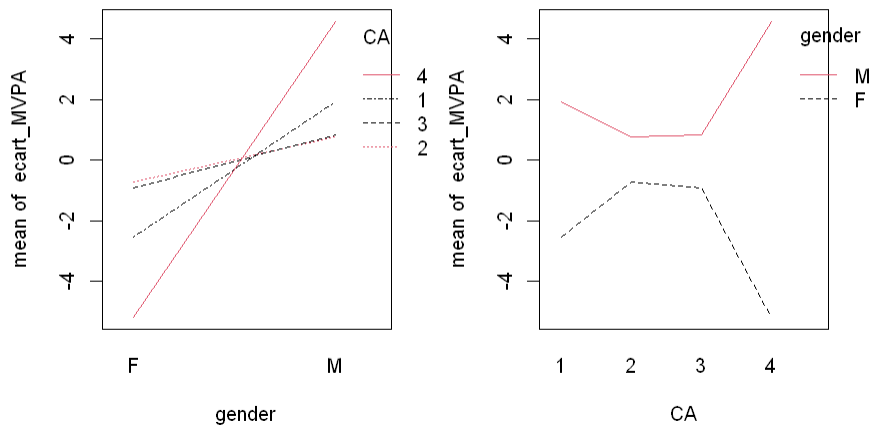
\includegraphics[width=\textwidth]{Interaction_1.PNG}
		\caption{Interactions entre les facteurs Genre et Champs d'apprentissage}
		\label{fig:interactions_1}
	\end{figure}
	On observe que les profils ne sont pas parallèles. La moyenne de \texttt{ecart\_MVPA} des filles ou des garçons diffère selon le champ d'apprentissage, et vice versa. Donc, ces graphiques suggèrent une interaction entre le genre et le champ d'apprentissage (CA).\\
	
	Avant d'examiner les résultats des tests associés au modèle, nous devons nous assurer que les conditions d'application du modèle sont remplies.\\


	
\item \textbf{Hypothèses du modèle} \\

\textbf{Indépendance} : l'hypothèse d'indépendance des observations est vérifiée (voir justification en section 3.2.1, partie b, Indépendance, page 16).\\

\textbf{Homoscédasticité} : la figure \ref{fig:variance2} présente le graphique de diagnostic pour l'homoscédasticité. Les valeurs prédites sont représentées en abscisse et les résidus en ordonnée. Ce graphique ne montre pas de tendance particulière, ce qui indique que la variance des résidus est relativement constante à travers tous les groupes. Donc l'hypothèse d'homoscédasticité peut être validée.\\
\begin{figure}[H]
	\centering
	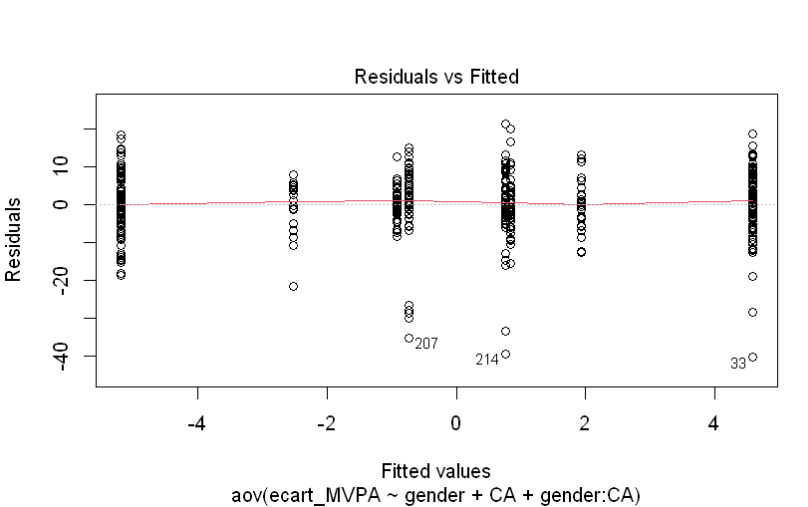
\includegraphics[width=\linewidth]{variance_2.PNG}
	\caption{Graphique de diagnostic de l'homoscédasticité pour le modèle M1}
	\label{fig:variance2}
\end{figure}

\textbf{Normalité des résidus} : la figure \ref{fig:QQplot_2} illustre le graphique quantiles contre quantiles (Q-Q plot).\\
\begin{figure}[H]
	\centering
	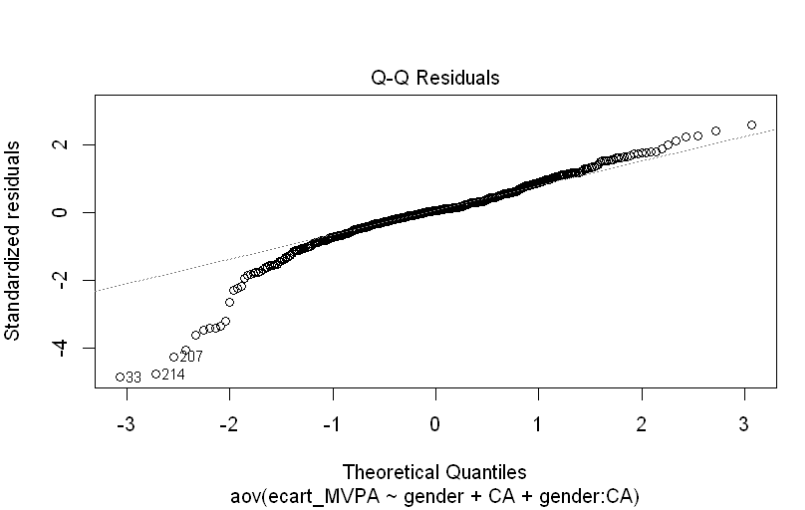
\includegraphics[width=\linewidth]{Normalité_2.PNG}
	\caption{Q-Q plot pour le modèle M1}
	\label{fig:QQplot_2}
\end{figure}
Les points sur la figure \ref{fig:QQplot_2} sont globalement alignés sur la ligne diagonale, à l'exception des extrémités de la distribution. De plus, avec 462 observations, l'ANOVA est relativement robuste à la non-normalité \cite{poulin2023}. Ces observations permettent de confirmer que l'hypothèse de normalité des résidus est raisonnable.



	\item \textbf{Résultats} \\
	
	Les hypothèses du modèle ayant été validées, nous pouvons maintenant présenter les résultats.\\
	
	\textbf{\textit{\underline{Test du modèle complet}}}\\
	
	Nous voulons tester les hypothèses suivantes :
	\begin{itemize}[label=--, leftmargin=*]
		\item \textbf{$H_0$} : $\alpha_i = 0$ et $\beta_j = 0$ et $\gamma_{ij} = 0 \quad \forall i, j$
		\item \textbf{$H_1$} : $\alpha_i \neq 0$ ou $\beta_j \neq 0$ ou $\gamma_{ij} \neq 0 \quad \forall  i, j$
	\end{itemize}
	
	La table \ref{tab:anova_results1} présente les résultats du test du modèle complet contre le modèle le plus simple.
	\begin{table}[H]
		\centering
		\caption{Tableau d'analyse de variance du modèle M1}
		\begin{tabular}{ccccccc}
			\toprule
			\textbf{Res.Df} & \textbf{RSS} & & \textbf{Df} & \textbf{Sum of Sq} & \textbf{F value} & \textbf{Pr(>F)} \\ 
			\midrule
			461 & 36916 & & & & & \\ 
			454 & 31593 & & 7 & 5323.2 & 10.928 & 8.944 $\times 10^{-13}$ \\ 
			\bottomrule
		\end{tabular}
		\label{tab:anova_results1}
	\end{table}
	La statistique de test est $F = \frac{\frac{SCE}{(IJ - 1)}}{\frac{SCR}{(n - IJ)}} = 10.928$ (la variabilité expliquée par le genre et le CA est 10.928 fois supérieure à la variabilité résiduelle). Sous $H_0$, $F$ suit une loi de Fisher avec $7$ et $454$ degrés de liberté, soit $F \sim \mathcal{F}_{7,454}$. La probabilité critique associée est de $8.944 \times 10^{-13}$ inférieur à 5\%, ce qui conduit au rejet de $H_0$. Il est à noter que l'ajustement du modèle n'est pas très satisfaisant, avec un coefficient de détermination $R^2 = 1 - \frac{31593}{36916} = 0.144$.\\
	
	\textbf{\textit{\underline{Test des sous-modèles}}} \\
	
	La table \ref{tab:anova_results2} présente les tests des effets des différents facteurs (genre, CA et leur interaction).\\
	\begin{table}[H]
		\centering
		\caption{Effets des différents facteurs (type II) dans le modèle M1}
		\begin{tabular}{lcccc}
			\toprule
			Source & Sum Sq & Df & F value & Pr(>F) \\ 
			\midrule
			genre & 3585.2 & 1 & 51.5200 & 2.911 $\times 10^{-12}$ \\ 
			CA & 6.4 & 3 & 0.0307 & 0.9927 \\ 
			genre:CA & 1738.0 & 3 & 8.3252 & 2.122 $\times 10^{-5}$ \\ 
			Résidus & 31592.8 & 454 & & \\ 
			\bottomrule
		\end{tabular}
		\label{tab:anova_results2}
	\end{table}
	
	\textit{Effet de l'interaction} : \\
	Nous testons les hypothèses suivantes :
	\begin{itemize}[label=--, leftmargin=*]
		\item \textbf{$H_0$} : $Y_{ijk} = \mu + \alpha_i + \beta_j + \epsilon_{ijk} \quad \forall i,j,k$ 
		\item \textbf{$H_1$} : $Y_{ijk} = \mu + \alpha_i + \beta_j + \gamma_{ij} + \epsilon_{ijk} \quad \forall i,j,k$
	\end{itemize}
	
	Pour le test de l'effet de l'interaction, la statistique de test est $F_{genre \times CA} = 8.3252$, qui, sous $H_0$, suit une loi de Fisher avec 3 et 454 degrés de liberté. La probabilité critique associée au test est de $2.122 \times 10^{-5}$. L'effet de l'interaction entre genre et CA est significatif au niveau de 5\%. Nous n'accorderons donc plus trop d'importance aux tests sur les facteurs principaux, car les deux facteurs principaux exercent leur influence par le biais de leur interaction.\\
	
	\textbf{\textit{\underline{Test de comparaison  de la moyenne de \texttt{ecart\_MVPA} des filles et garçons selon le champ d'apprentissage}}} \\
	
	Nous avons détecté un effet significatif de l'interaction et nous nous intéressons donc à la différence de moyenne de \texttt{ecart\_MVPA} entre les filles et les garçons selon les différents CA. Nous voulons tester les hypothèses suivantes :	
	\begin{itemize}[label=--, leftmargin=*]
		\item $H_0 : \theta_{i_1j} = \theta_{i_2j}$
		\item $H_1 : \theta_{i_1j} \neq \theta_{i_2j}$
	\end{itemize}
	où $\theta_{i_1j_1}$ et $\theta_{i_2j_2}$ sont les moyennes dans chaque groupe différent et $i_1, i_2 \in \{1, 2\}$ avec $i_1 \neq i_2$ ; $j \in \{1, \ldots, 4\}$. \\
	
	La table \ref{tab:ecarts_mvpa_1} présente les tests de comparaison des moyennes de \texttt{ecart\_MVPA} (tests post hoc de Tukey-Kramer) entre les filles et garçons selon les différents champs d'apprentissage (CA).\\
	\begin{table}[H]
		\centering
		\caption{Test de comparaison des moyennes de \texttt{ecart\_MVPA} des filles et garçons dans les différents CA}
		\begin{tabular}{|p{5cm}|c|c|c|c|}
			\hline
			& CA1 & CA2 & CA3 & CA4 \\ 
			\hline
			Écart moyen entre filles et garçons des écarts à la moyenne de MVPA de chaque classe & -4.4548 & -1.4898 & -1.7470 & -9.7647 \\ 
			\hline
			Intervalle de confiance & -12.010 à 3.100 & -6.4730 à 3.493 & -6.759 à 3.265 & -13.286 à -6.244 \\ 
			\hline
			P-valeur & 0.6235 & 0.9850 & 0.9600 & 0.0000 \\ 
			\hline
		\end{tabular}
		\label{tab:ecarts_mvpa_1}
	\end{table}
	
	
	La moyenne de \texttt{ecart\_MVPA} des garçons est significativement supérieur à celui des filles dans le champ 4 (p-valeur < 0.05, on rejette $H_0$). En revanche, dans les autres champs, cette différence n'est pas significative avec des p-valeurs largement supérieures à 5\% (nous conservons $H_0$). \\
	
	La figure \ref{fig:Test post hoc_garphe_1} présente un diagramme en barres qui représente les écarts de moyenne de \texttt{ecart\_MVPA} entre les filles et les garçons selon le CA, avec l'écart-type et les p-valeurs associées.\\
	
	\begin{figure}[H]
		\centering
		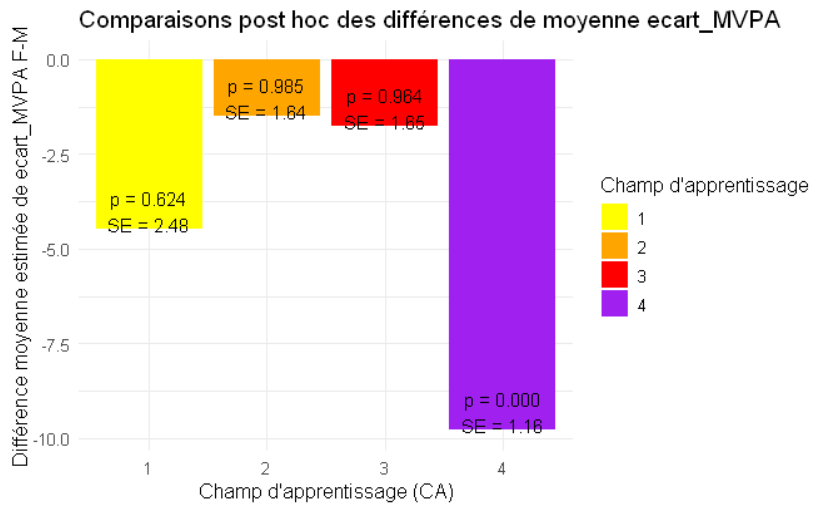
\includegraphics[width=\linewidth]{Diagramme_1.PNG}
		\caption{Diagramme en barres représentatif des tests de comparaison des moyennes de \texttt{ecart\_MVPA} des filles et garçons dans les différents CA avec les p-valeurs et écarts-types}
		\label{fig:Test post hoc_garphe_1}
	\end{figure}

	
\textbf{\textit{\underline{Taille d'effet}}}\\

Dans le champ 4, nous avons observé une différence significative de la moyenne de \texttt{ecart\_MVPA} entre les filles et les garçons, ce qui se traduit par un effet significatif de l'interaction entre le genre et le champ d'apprentissage (CA). Nous souhaitons maintenant évaluer la force de cet effet.\\
La table \ref{table:effect_size_2} présente les valeurs de la mesure de la taille d'effet ($\omega^2$) pour chaque facteur, ainsi que les intervalles de confiance unilatéraux à 95\%.\\

\begin{table}[H]
	\centering
	\caption{Tailles d'effet ($\omega^2$) et intervalles de confiance à 95\% (unilatéraux)}
	\begin{tabular}{ccc}
		\toprule
		Paramètre & $\omega^2$ & 95\% CI \\
		\midrule
		Genre & 0.10 & [0.06, 1.00] \\
		CA & 0.00 & [0.00, 1.00] \\
		Genre:CA & 0.05 & [0.02, 1.00] \\
		\bottomrule
	\end{tabular}
	\label{table:effect_size_2}
\end{table}

La taille d'effet pour l'interaction entre le genre et le CA est de 0,05, ce qui signifie que 5\% de la variance totale de la variable dépendante (\texttt{ecart\_MVPA}) peut être attribuée à l'effet de l'interaction. Bien que cette taille d'effet soit modérée, elle suggère que les différences observées peuvent avoir une importance pratique. En éducation physique, même de faibles écarts peuvent avoir un impact significatif sur le long terme. Par conséquent, il est pertinent de tenir compte de l'écart d'engagement entre les filles et les garçons observé dans le champ 4 dans la pratique.

\end{enumerate}

\subsubsection{Examen de l'écart de MVPA entre Filles et Garçons selon la catégorie IPS}
L'objectif dans cette partie est d'examiner l'effet du genre et de la catégorie IPS sur le niveau d'engagement physique en EPS. Nous utilisons donc un modèle d'ANOVA à deux facteurs (genre et catégorie IPS) avec comme variable dépendante \texttt{ecart\_MVPA}. Pour la contrainte sur le modèle, nous adoptons celle de la somme nulle. Le modèle est formulé comme suit :
\begin{equation}
	Y_{ijk} = \mu + \alpha_i + \beta_j + \gamma_{ij} + \epsilon_{ijk},\quad \epsilon_{ijk} \overset{\text{i.i.d}}{\sim} \mathcal{N}(0,\sigma^2)\tag{M2}
\end{equation}
$\quad i = 1, \ldots, 2, \quad j = 1, \ldots, 3$
où $\mu$ est l'effet moyen général, $\alpha_i$ représente l'effet principal du genre, $\beta_j$ représente l'effet principal de la catégorie IPS, $\gamma_{ij}$ le terme d'interaction, et $\epsilon_{ijk}$ les résidus, avec $k$ étant l'indice de répétition pour le couple $(i,j)$. Enfin, $\sigma^2$ est la variance résiduelle.



\begin{enumerate}[label=\textbf{\alph*})]
	\item \textbf{Plan et visualisation des données} \\
	
	Le tableau \ref{table:contingence_2} présente la répartition des observations dans les différents groupes (croisement entre la catégorie d'IPS et le genre). 
	\begin{table}[H]
		\centering
		\caption{Tableau de contingence entre le genre et la catégorie IPS}
		\begin{tabular}{cccc}
			\toprule
			& Élevée & Faible & Moyenne \\
			\midrule
			F & 93 & 48 & 79 \\
			M & 89 & 44 & 109 \\
			\bottomrule
		\end{tabular}
		\label{table:contingence_2}
	\end{table}
	On observe que les effectifs varient d'un groupe à l'autre, ce qui signifie que nos données ne sont pas équilibrées. Nous avons donc recours à une ANOVA de Type II. En effet, dans le cadre de notre étude, l'ordre d'insertion des facteurs dans le modèle n'est pas crucial.\\
	
La table \ref{tab:desc_stats_ips} présente les statistiques descriptives pour les différents groupes.
\begin{table}[H]
	\centering
	\caption{Statistiques descriptives par genre et catégorie IPS}
	\begin{tabular}{ccrcccc}
		\toprule
		\textbf{Genre} & \textbf{Catégorie IPS} & \textbf{Effectif} & \textbf{Moyenne} & \textbf{Écart-type} & \textbf{Min} & \textbf{Max} \\
		\midrule
		F & Élevée & 60 & -1.932 & 9.485 & -30.776 & 14.224 \\
		F & Faible & 44 & -2.733 & 8.840 & -24.042 & 10.198 \\
		F & Moyenne & 73 & -4.426 & 7.835 & -23.893 & 13.310 \\
		M & Élevée & 55 & 3.918 & 8.613 & -32.776 & 23.417 \\
		M & Faible & 39 & 2.630 & 6.360 & -14.033 & 12.958 \\
		M & Moyenne & 100 & 2.591 & 9.175 & -35.857 & 20.885 \\
		\bottomrule
	\end{tabular}
	\label{tab:desc_stats_ips}
\end{table}
On observe des différences de moyenne de \texttt{ecart\_MVPA} entre les filles et les garçons au sein d'une même catégorie d'IPS. Nous aimerions donc savoir si ces différences observées sont significatives.\\


\textit{\textbf{\underline{Représentation graphique des interactions}}}\\

La figure \ref{fig:interactions_2} montre les graphes des interactions entre les facteurs genre et catégorie IPS.
\begin{figure}[h!]
	\centering
	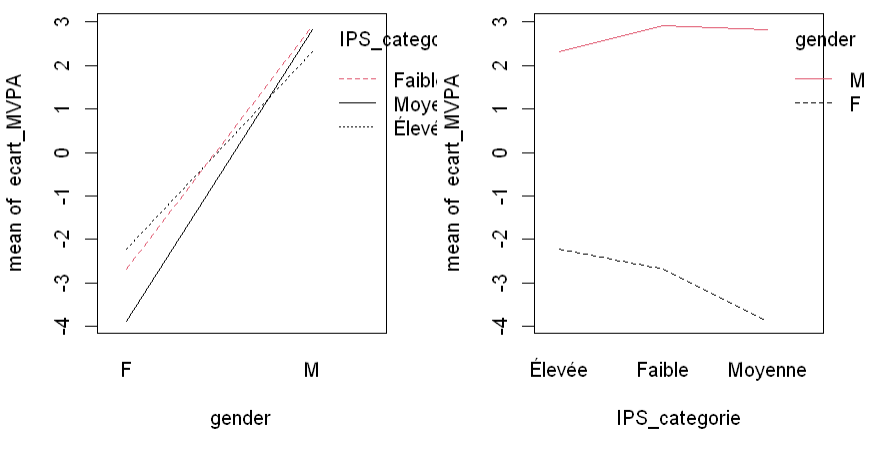
\includegraphics[width=\textwidth]{Interaction_2.PNG}
	\caption{Interactions entre les facteurs Genre et Catégorie IPS}
	\label{fig:interactions_2}
\end{figure}
On remarque que les profils ne sont pas exactement parallèles mais quasiment. La moyenne de \texttt{ecart\_MVPA} des filles ou des garçons ne diffère pas trop selon la catégorie IPS, et vice versa. Donc, ces graphiques suggèrent une très légère interaction entre le genre et la catégorie IPS.\\

Avant d'examiner les résultats, nous devons nous assurer que les conditions d'application du modèle sont respectées.\\

	
\item \textbf{Hypothèses du modèle} \\

\noindent
\textbf{Indépendance} : l'hypothèse d'indépendance des observations est vérifiée (voir justification en section 3.2.1, partie b, Indépendance, page 16).\\

\noindent
\textbf{Homoscédasticité} : pour valider l'hypothèse d'homoscédasticité, nous visualisons le graphe des résidus en fonction des valeurs prédites, présenté dans la figure \ref{fig:variance2}.
\begin{figure}[H]
	\centering
	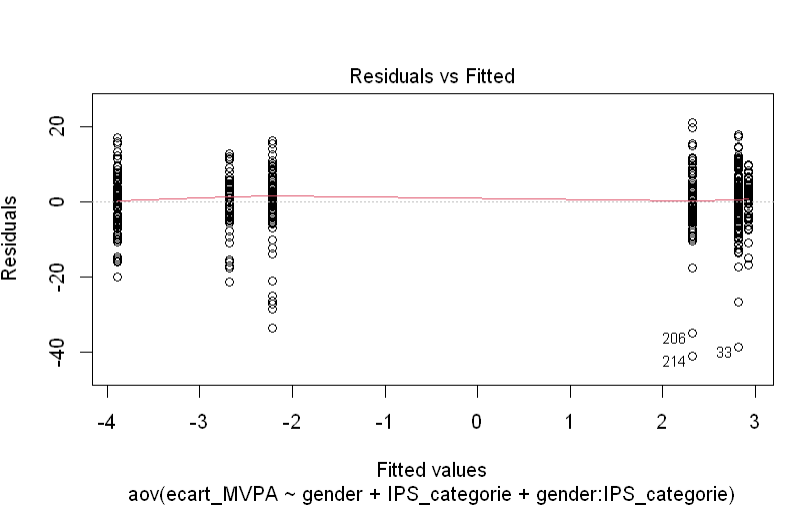
\includegraphics[width=\linewidth]{variance_3.PNG}
	\caption{Graphique de diagnostic de l'homoscédasticité pour le modèle M2}
	\label{fig:variance2}
\end{figure}
La figure \ref{fig:variance2} montre que le nuage de points ne présente pas de tendance particulière, ce qui suggère que la variance des résidus est similaire dans tous les groupes, confirmant ainsi l'homoscédasticité.\\

\noindent
\textbf{Normalité des résidus} : la figure \ref{fig:QQplot_3} présente le graphique quantiles contre quantiles (Q-Q plot). Les points sur le graphique sont globalement alignés sur la ligne diagonale, à l'exception des extrémités. De plus, avec 462 observations, l'ANOVA est relativement robuste à la non-normalité \cite{poulin2023}. Ces observations confirment que l'hypothèse de normalité des résidus est raisonnable.

\begin{figure}[H]
	\centering
	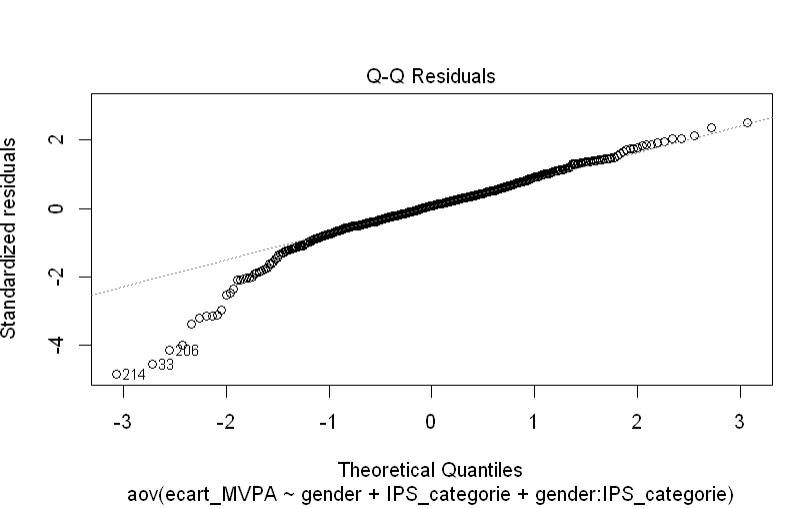
\includegraphics[width=\linewidth]{Normalité_3.PNG}
	\caption{Q-Q plot pour le modèle M2}
	\label{fig:QQplot_3}
\end{figure}


	\noindent
	\item \textbf{Résultats} \\
	
	Les hypothèses du modèle ayant été validées, nous pouvons maintenant présenter les résultats. \\
	
	\noindent
	\textbf{\textit{\underline{Test du modèle complet}}}  \\
	
	Nous testons les hypothèses suivantes :
	\begin{itemize}[label=--, leftmargin=*]
		\item \textbf{$H_0$} : $\alpha_i = 0$ et $\beta_j = 0$ et $\gamma_{ij} = 0 \quad \forall i,j$
		\item \textbf{$H_1$} : $\alpha_i \neq 0$ ou $\beta_j \neq 0$ ou $\gamma_{ij} \neq 0 \quad \forall i,j$
	\end{itemize}
	
	La table \ref{table:analyse_variance_2} présente les résultats du test du modèle complet par rapport au modèle le plus simple.
	
	\begin{table}[H]
		\centering
		\caption{Tableau d'analyse de variance pour le modèle M2}
		\begin{tabular}{rrrrrrr}
			\toprule
			\textbf{Res.Df} & \textbf{RSS} & \textbf{Df} & \textbf{Sum of Sq} & \textbf{F} & \textbf{Pr(>F)} \\ 
			\midrule
			461 & 36916 & & & & \\ 
			456 & 33199 & 5 & 3717.1 & 10.211 & 2.74e-09 *** \\ 
			\bottomrule
		\end{tabular}
		\label{table:analyse_variance_2}
	\end{table}
	
	La statistique de Fisher est $F = \frac{\frac{SCE}{(IJ - 1)}}{\frac{SCR}{(n - IJ)}} = 10.211$, ce qui signifie que la variabilité expliquée par le genre et la catégorie d'IPS est environ 10 fois supérieure à la variabilité résiduelle. Sous $H_0$, $F$ suit une loi de Fisher avec $5$ et $456$ degrés de liberté. La p-valeur obtenue est de $2.74 \times 10^{-9}$, ce qui est bien inférieur à 5\%, nous rejetons donc $H_0$. Cependant, l'ajustement du modèle n'est pas particulièrement satisfaisant, avec un $R^2 = 1 - \frac{33199}{36916} = 0.1006$. \\
	
	\noindent
	\textbf{\textit{\underline{Test des sous-modèles}}}  \\
	
	La table \ref{tab:anova_results3} présente les résultats des tests pour les effets individuels des facteurs (genre, catégorie d'IPS et leur interaction).
	
	\begin{table}[H]
		\centering
		\caption{Effets des différents facteurs (type II) dans le modèle M2}
		\begin{tabular}{lrrrr}
			\toprule
			Source & Sum Sq & Df & F value & Pr(>F) \\ 
			\midrule
			gender                & 3610   & 1  & 49.5860 & 7.028e-12 *** \\ 
			IPS\_categorie        & 31     & 2  & 0.2152  & 0.8064    \\ 
			gender:IPS\_categorie & 107    & 2  & 0.7349  & 0.4801    \\ 
			Residuals             & 33199  & 456 &         &           \\ 
			\bottomrule
		\end{tabular}
		\label{tab:anova_results3}
	\end{table}
	
	\noindent
	\textit{Effet de l'interaction} : \\
	Nous testons les hypothèses suivantes :
	\begin{itemize}[label=--, leftmargin=*]
		\item \textbf{$H_0$} : $Y_{ijk} = \mu + \alpha_i + \beta_j + \epsilon_{ijk} \quad \forall i,j,k$ 
		\item \textbf{$H_1$} : $Y_{ijk} = \mu + \alpha_i + \beta_j + \gamma_{ij} + \epsilon_{ijk} \quad \forall i,j,k$
	\end{itemize}
	
	Pour le test de l'effet de l'interaction, la statistique de test est $F_{gender \times IPS\_categorie} = 0.7349$, qui suit une loi de Fisher avec $2$ et $456$ degrés de liberté sous $H_0$. La p-valeur associée est de 0.4801 supérieur au seuil de 5\%, donc nous conservons $H_0$, indiquant qu'il n'y a pas d'interaction significative entre le genre et la catégorie d'IPS. \\
	
	\noindent
	\textit{Effet de la catégorie d'IPS} : \\
	Nous testons si la catégorie d'IPS a un effet sur \texttt{ecart\_MVPA}. Nous testons les hypothèses suivantes :
	\begin{itemize}[label=--, leftmargin=*]
		\item \textbf{$H_0$} : $Y_{ijk} = \mu + \alpha_i + \epsilon_{ijk} \quad \forall i,j,k$ 
		\item \textbf{$H_1$} : $Y_{ijk} = \mu + \alpha_i + \beta_j + \epsilon_{ijk} \quad \forall i,j,k$
	\end{itemize}
	
	La statistique de test pour l'effet de la catégorie d'IPS est $F_{IPS\_categorie} = 0.2152$, qui suit une loi de Fisher avec $2$ et $456$ degrés de liberté sous $H_0$. La p-valeur observée est de 0.8064 supérieur à 5\%, donc nous conservons $H_0$, ce qui signifie qu'il n'y a pas d'effet significatif de la catégorie d'IPS sur \texttt{ecart\_MVPA}. \\
	
	Ainsi, l'écart d'engagement entre filles et garçons en EPS ne dépend pas de la catégorie socioprofessionnelle de l'établissement.\\
	

\end{enumerate}

\subsubsection{Examen de l'écart de MVPA entre Filles et Garçons selon le milieu géographique}
Afin d'évaluer l'effet des variables genre et milieu géographique sur le niveau d'engagement physique en EPS, nous utilisons une ANOVA à deux facteurs avec comme variable dépendante \texttt{ecart\_MVPA}. Le modèle à tester, en respectant la contrainte de somme nulle, est spécifié comme suit : 
\begin{equation}
	Y_{ijk} = \mu + \alpha_i + \beta_j + \gamma_{ij} + \epsilon_{ijk}, \quad \epsilon_{ijk} \overset{\text{i.i.d}}{\sim} \mathcal{N}(0,\sigma^2)\tag{M3}
\end{equation}
$\quad i = 1, \ldots, 2, \quad j = 1, \ldots, 4$
avec un effet moyen général $\mu$, $\alpha_i$ représente l'effet principal du genre, $\beta_j$ représente l'effet principal du milieu géographique, un terme d'interaction $\gamma_{ij}$, les résidus $\epsilon_{ijk}$ avec $k$ l'indice de répétition pour le couple $(i,j)$ et $\sigma^2$ est la variance résiduelle.\\

\begin{enumerate}[label=\textbf{\alph*})]
\item \textbf{Plan et Visualisation des données}  \\

\noindent
La table \ref{tab:tab_contingence_3} présente les effectifs pour chaque combinaison de genre et de milieu géographique. 

\begin{table}[H]
	\centering
	\caption{Tableau de contingence des effectifs par genre et milieu géographique}
	\begin{tabular}{ccc}
		\toprule
		& Rural & Urbain \\
		\midrule
		F & 101 & 119 \\
		M & 102 & 140 \\
		\bottomrule
	\end{tabular}
	\label{tab:tab_contingence_3}
\end{table}

\noindent
Les effectifs ne sont pas parfaitement équilibrés entre les groupes. En raison de cette disparité, nous utiliserons une ANOVA de type II, où l'ordre des facteurs n'affecte pas les résultats. \\

\noindent
La table \ref{tab:desc_stats_4} fournit des statistiques descriptives pour les différents groupes, en fonction du genre et du milieu géographique.

\begin{table}[H]
	\centering
	\caption{Statistiques descriptives par genre et milieu géographique}
	\begin{tabular}{ccrcccc}
		\toprule
		\textbf{Genre} & \textbf{Géographie} & \textbf{Effectif} & \textbf{Moyenne\_écart\_MVPA} & \textbf{Écart-type} & \textbf{Min} & \textbf{Max} \\
		\midrule
		F & Rural & 66 & -0.658 & 8.969 & -30.776 & 14.224 \\
		F & Urbain & 111 & -4.647 & 8.211 & -24.042 & 13.310 \\
		M & Rural & 67 & 1.940 & 8.547 & -32.776 & 22.224 \\
		M & Urbain & 127 & 3.521 & 8.459 & -35.857 & 23.417 \\
		\bottomrule
	\end{tabular}
	\label{tab:desc_stats_4}
\end{table}

\noindent
On observe une différence notable dans les moyennes de \texttt{ecart\_MVPA} entre les filles et les garçons en milieu urbain, tandis que la différence est beaucoup plus faible en milieu rural. Ces observations suggèrent des variations potentielles qui méritent d'être examinées pour leur signification statistique. \\


\textit{\textbf{\underline{Représentation graphique des interactions}}}\\

Les graphiques des interactions entre les facteurs genre et milieu géographique, présentés dans la figure \ref{fig:interactions_3}, montrent que les profils ne sont pas parallèles. La moyenne de \texttt{ecart\_MVPA} des filles ou des garçons diffère selon le milieu géographique, et vice versa. Ces graphiques suggèrent une interaction entre le genre et le milieu géographique.\\

\begin{figure}[H]
	\centering
	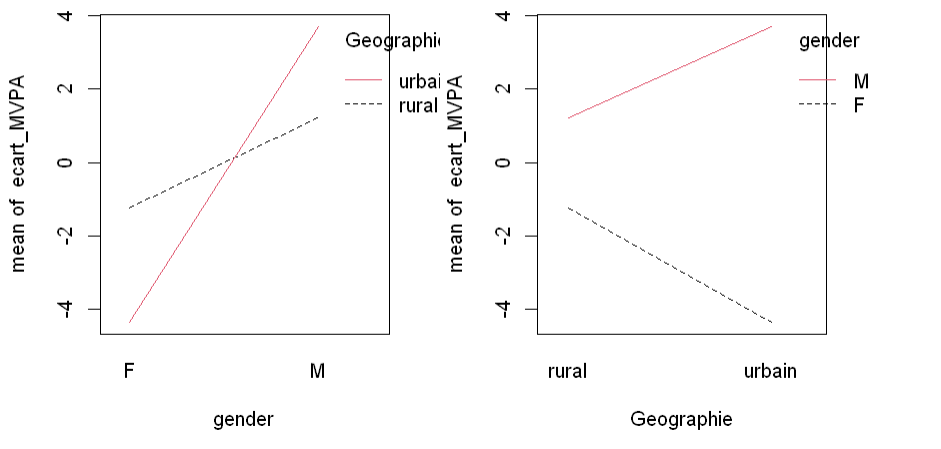
\includegraphics[width=\textwidth]{Interaction_3.PNG}
	\caption{Interactions entre les facteurs Genre et Milieu géographique}
	\label{fig:interactions_3}
\end{figure}

\noindent
Avant d'examiner les résultats des tests associés au modèle M3, il est essentiel de vérifier que les conditions d'application du modèle sont respectées.

	
\item \textbf{Hypothèses du modèle} \\

\noindent
\textbf{Indépendance} : l'hypothèse d'indépendance des observations est vérifiée (voir justification, section 3.2.1, partie b, sur l'indépendance page 16).\\

\noindent
\textbf{Homoscédasticité} : l'hypothèse d'homoscédasticité, qui stipule que les variances des résidus doivent être égales à travers les différents groupes, est examinée à l'aide du graphique présenté dans la figure \ref{fig:variance3}. Ce graphique illustre la dispersion des résidus par rapport aux valeurs ajustées. Le nuage de points ne montre pas de tendance particulière, ce qui indique que la distribution des résidus semble homogène et que l'hypothèse d'homoscédasticité est raisonnable.
\begin{figure}[H]
	\centering
	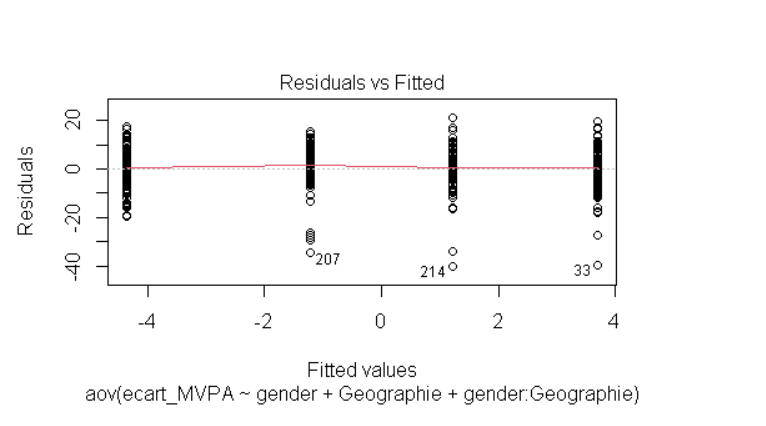
\includegraphics[width=\linewidth]{variance_4.PNG}
	\caption{Graphique de diagnostic de l'homoscédasticité pour le modèle M3}
	\label{fig:variance3}
\end{figure}

\noindent
\textbf{Normalité des résidus} : la figure \ref{fig:qq_plot4} montre le graphique quantiles contre quantiles (Q-Q plot) des résidus. Les points sur ce graphique sont globalement alignés sur la ligne de référence, bien que des écarts puissent être observés aux queues de distribution. De plus, l'ANOVA est connue pour être relativement robuste à la non-normalité avec une grande taille d'échantillon (462 observations) \cite{poulin2023}. Ainsi, l'hypothèse de normalité des résidus est considérée comme raisonnable dans ce contexte.
\begin{figure}[H]
	\centering
	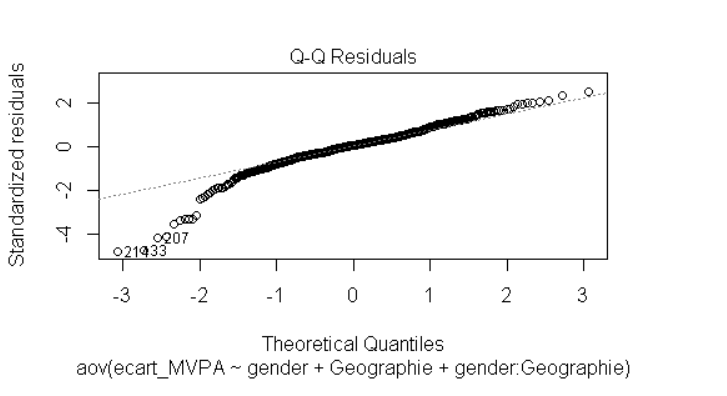
\includegraphics[width=\linewidth]{Normalité_4.PNG}
	\caption{Q-Q plot des résidus pour le modèle M3}
	\label{fig:qq_plot4}
\end{figure}

	
	\item \textbf{Résultats} \\
	
	Les hypothèses du modèle ayant été validées, nous pouvons maintenant présenter les résultats. \\
	
	\noindent
	\textbf{\textit{\underline{Test du modèle complet}}} \\
	
	Le test du modèle complet consiste à comparer le modèle le plus simple (modèle constant) au modèle complet. Les résultats sont présentés dans la table \ref{tab:anova_results_3}. Nous testons les hypothèses suivantes :
	\begin{itemize}[label=--, leftmargin=*]
		\item $H_0 : \alpha_i = 0$ et $\beta_j = 0$ et $\gamma_{ij} = 0 \quad \forall i,j$ 
		\item $H_1 : \alpha_i \neq 0$ ou $\beta_j \neq 0$ ou $\gamma_{ij} \neq 0 \quad \forall i,j$ 
	\end{itemize}

	\begin{table}[H]
		\centering
		\caption{Tableau d'analyse de variance du modèle M3}
		\begin{tabular}{rrrrrl}
			\toprule
			\textbf{Res.Df} & \textbf{RSS} & \textbf{Df} & \textbf{Sum of Sq} & \textbf{F} & \textbf{Pr(>F)} \\
			\midrule
			461 & 36916 &    &         &         &        \\
			458 & 32439 &  3 & 4477.3  & 21.072  & 8.375e-13 *** \\
			\bottomrule
		\end{tabular}
		\label{tab:anova_results_3}
	\end{table}
	La statistique de test est $F = \frac{\frac{SCE}{3}}{\frac{SCR}{458}} = 21.072$, donc la variabilité expliquée par le genre et le milieu géographique est 21 fois supérieure à la variabilité résiduelle. Sous $H_0$, $F \sim \mathcal{F}_{3,458}$. La p-valeur associée est $8.375 \times 10^{-13}$ inférieur à 0.05, ce qui nous conduit à rejeter $H_0$. Cependant, l'ajustement du modèle n'est pas très satisfaisant, avec un $R^2 = 1 - \frac{32439}{36916} = 0.1212$. \\
	
	\noindent
	\textbf{\textit{\underline{Test des sous-modèles}}} \\
	
	Les tests des effets des différents facteurs sont présentés dans la table \ref{tab:test_effet_M3}. 
	\begin{table}[H]
		\centering
		\caption{Effet des différents facteurs (type II) dans le modèle M3}
		\begin{tabular}{lrrrr}
			\toprule
			& Sum Sq & Df & F value & Pr(>F)     \\
			\midrule
			gender            & 3584   & 1  & 50.6006 & 4.386e-12  \\
			Geographie        & 5      & 1  & 0.0725  & 0.7879     \\
			gender:Geographie & 893    & 1  & 12.6145 & 0.0004224  \\
			Residuals         & 32439  & 458 &         &            \\
			\bottomrule
		\end{tabular}
		\label{tab:test_effet_M3}
	\end{table}
	
	\noindent
	\textit{Effet de l'interaction} : \\
	Nous testons les hypothèses suivantes :
	\begin{itemize}[label=--, leftmargin=*]
		\item \textbf{$H_0$} : $Y_{ijk} = \mu + \alpha_i + \beta_j + \epsilon_{ijk} \quad \forall i,j,k$ 
		\item \textbf{$H_1$} : $Y_{ijk} = \mu + \alpha_i + \beta_j + \gamma_{ij} + \epsilon_{ijk} \quad \forall i,j,k$
	\end{itemize}
	La statistique de test pour l'effet d'interaction $F_{gender*Geographie} = 12.6145$, qui sous $H_0$ suit une loi de Fisher à 1 et 458 ddl. La p-valeur associée est 0.0004224. Cette p-valeur étant inférieure à 0.05, nous rejetons $H_0$. L'effet de l'interaction entre genre et milieu géographique est significatif. Les deux facteurs influencent le MVPA principalement à travers leur interaction, il n'est donc pas nécessaire de tester leur effet principal séparément.\\
	
	\noindent
	\textbf{\textit{\underline{Test de comparaison  de la moyenne de \texttt{ecart\_MVPA} des filles et garçons selon le milieu géographique}}} \\
	
	Un effet significatif de l'interaction est détecté et ici nous sommes intéressés par la différence de moyenne de \texttt{ecart\_MVPA} entre les filles et garçons selon les différents milieux géographiques. Nous voulons tester les hypothèses : 
	\begin{itemize}[label=--, leftmargin=*]
		\item $H_0 : \theta_{i_1j} = \theta_{i_2j}$
		\item $H_1 : \theta_{i_1j} \neq \theta_{i_2j}$
	\end{itemize}
	où $\theta_{i_1j_1}$ et $\theta_{i_2j_2}$ sont les moyennes de \texttt{ecart\_MVPA} dans chaque groupe différent et $i_1,i_2\in{\{1, 2\}} $ avec $ i_1 \neq i_2$ ; $j\in{\{1,2\}}$.\\
	la table \ref{tab:ecarts_mvpa_genre_localisation} présente la comparaison de moyenne de \texttt{ecart\_MVPA} des filles et garçons selon le milieu géographique.
	\begin{table}[H]
		\centering
		\caption{Tests de comparaison de moyenne de \texttt{ecart\_MVPA} des filles et garçons selon le milieu géographique}
		\begin{tabular}{|p{5cm}|c|c|}
			\hline
			& Rural & Urbain \\ 
			\hline
			Écart entre filles et garçons des écarts à la moyenne de MVPA de chaque classe & -2.44 & -8.06 \\ 
			\hline
			Intervalle de confiance & -5.49 à 0.602 & -10.761 à -5.350 \\ 
			\hline
			P-valeur & 0.1650 & 0.000 \\ 
			\hline
		\end{tabular}
		
		\label{tab:ecarts_mvpa_genre_localisation}
	\end{table}
	
	La moyenne de \texttt{ecart\_MVPA} des garçons est significativement supérieur à celui des filles en milieu urbain (p-valeur <.05, nous rejetons $H_0$) par contre en milieu rural cette différence n'est pas significative (p-valeur > .05, nous conservons $H_0$). \\
	
	La figure \ref{fig:Test post hoc_2} présente un diagramme en barre qui représente les écart de moyenne de ecart\_MVPA entre les filles et garçons selon le milieu géographique avec l'écart type et les p-valeurs associé.
	
	\begin{figure}[H]
		\centering
		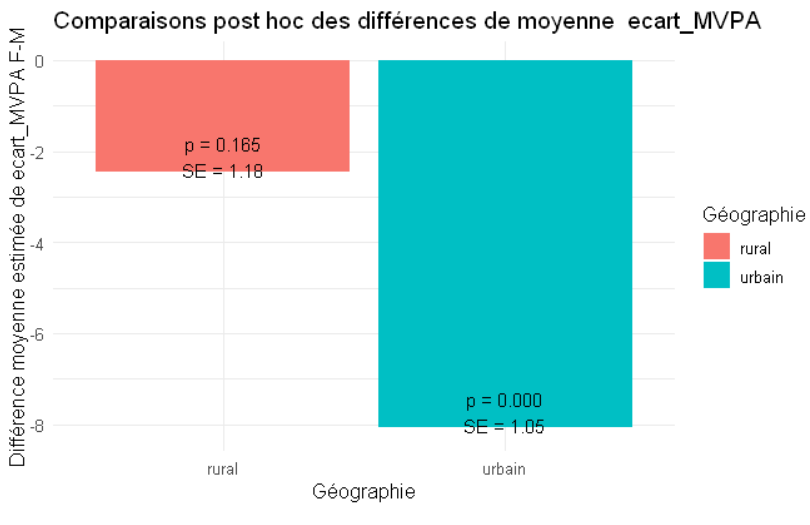
\includegraphics[width=\linewidth]{Diagramme_2.PNG}
		\caption{Diagramme en barre représentatif des tests de comparaison des moyennes de \texttt{ecart\_MVPA} des filles et garçons dans les différents milieu géographiques avec les p-valeurs et écart-type}
		\label{fig:Test post hoc_2}
	\end{figure}
	
	\noindent
\textbf{\textit{\underline{Taille d'effet}}} \\

En milieu urbain, nous avons observé une différence significative de moyenne de \texttt{ecart\_MVPA} entre filles et garçons, ce qui est traduit par un effet significatif de l'interaction entre le genre et le milieu géographique. La question qui se pose maintenant est celle de la force de cet effet. \\
La table \ref{table:effect_size_3} présente les valeurs de la mesure de la taille d'effet ($\omega^2$) pour chaque facteur.
\begin{table}[H]
	\centering
	\caption{Tableau des tailles d'effet $\omega^2$ et intervalles de confiance à 95\% (unilatéraux)}
	\begin{tabular}{|l|c|c|}
		\hline
		\textbf{Paramètre} & \textbf{$\omega^2$} & \textbf{95\% CI} \\
		\hline
		gender             & 0.10                      & [0.06, 1.00]      \\
		Geographie         & 0.00                      & [0.00, 1.00]      \\
		gender:Geographie  & 0.02                      & [0.01, 1.00]      \\
		\hline
	\end{tabular}
	\label{table:effect_size_3}
\end{table}

La taille d'effet pour l'interaction entre le genre et le milieu géographique est $\omega^2 = 0.02$, ce qui indique que 2\% de la variance totale de la variable dépendante (\texttt{ecart\_MVPA}) peut être attribuée à l'effet de l'interaction. Bien que cette taille d'effet soit relativement faible, elle suggère que l'interaction entre le genre et le milieu géographique a une influence pratique et non négligeable sur l'\textit{ecart\_MVPA}, surtout en éducation physique, où une faible taille d'effet peut avoir un impact significatif sur le long terme. Donc, la différence de moyenne observée entre filles et garçons en milieu urbain est bien réelle et doit être considérée dans la pratique.

\end{enumerate}

\subsection{Discussion sur les limites des résultats}

Il est important de noter que les données déséquilibrées entre différents groupes (par exemple, un nombre de participants plus élevé dans certaines catégories que dans d'autres) peuvent influencer les résultats des analyses statistiques. Bien que 462 observations soient relativement importantes, la taille de l'échantillon dans certains sous-groupes (par exemple, certains champs d'apprentissage ou certaines catégories socioculturelles) peut être limitée. Cela peut réduire la puissance des tests et accroître l'incertitude des estimations.

Les participants ont été recrutés parmi les élèves ayant rendu les autorisations parentales et souhaitant participer à l'étude. Cela peut introduire un biais de sélection si les élèves plus motivés ou ayant un meilleur accès aux ressources éducatives sont surreprésentés.

Le calcul et l'interprétation des tailles d'effet dans le cas de plans non équilibrés sont plus complexes, car une partie de la variance est manquante. En effet, lorsque la variabilité totale ne peut pas être entièrement décomposée en variabilité des différents effets, certaines variabilités non attribuables à un effet spécifique disparaissent dans le cadre de l'ANOVA de type II ou III. Ainsi, bien que la taille d'effet puisse ne pas être aussi précise dans les plans non équilibrés, elle fournit néanmoins une vue d'ensemble sur la force de l'effet du facteur, pour autant que le plan ne soit pas trop déséquilibré.

Les résultats de cette étude sont basés sur des données recueillies en Alsace et en Île-de-France. La généralisation de ces résultats à d'autres régions de France doit être effectuée avec prudence.

Enfin, le fait d'avoir examiné le niveau d'engagement physique en EPS en se basant sur l'écart de MVPA par rapport à la moyenne de MVPA de chaque classe ne permet pas de prendre en compte les effets aléatoires liés aux collèges et aux classes appartenant à ces collèges, qui sont bien présents dans notre population.


\newpage
\section*{Conclusion}
\sectionmark{Conclusion}
\addcontentsline{toc}{section}{Conclusion}
L'objectif de cette étude était d'examiner les écarts d'engagement physique entre les filles et les garçons lors d'un cours d'EPS de 2 heures en tenant compte de divers facteurs : le champ d'activité, la catégorie socioculturelle de l'établissement (IPS) et le milieu géographique. Les résultats montrent une implication généralement plus élevée des garçons par rapport aux filles.\\
Les écarts d'engagement varient selon le champ d'apprentissage. Une différence significative a été observée uniquement dans le champ 4, dédié aux activités d'opposition. En revanche, dans les autres champs (sports de performance, sports de plein air et activités artistiques), les différences entre les sexes ne sont pas significatives. Concernant les catégories d'IPS des établissements scolaires, aucune influence notable de la catégorie socioculturelle sur les écarts d'engagement entre les sexes n'a été détectée. Cependant, le milieu géographique joue un rôle important : en milieu urbain, les garçons s'impliquent significativement plus que les filles, tandis que cette différence n'est pas significative en milieu rural. Cela suggère que des facteurs contextuels spécifiques pourraient influencer les écarts d'engagement physique dans ces environnements.\\
Ces résultats soulignent l'importance de prendre en compte les contextes écologiques et socioculturels pour promouvoir l'activité physique dans les établissements scolaires. Ils mettent également en évidence la nécessité de développer des stratégies ciblées pour encourager l'engagement des filles, en particulier dans les milieux urbains et certains champs d'apprentissage.\\
En outre, ce stage m'a permis de développer des compétences pratiques en analyse de données statistiques, telles que l'utilisation de l'ANOVA à deux facteurs avec plan non équilibré. J'ai appris à gérer des données déséquilibrées et à interpréter les résultats tout en tenant compte des biais potentiels. La rédaction d'un article scientifique a également renforcé mes compétences en communication des résultats de recherche. De plus, j'ai acquis des compétences précieuses en gestion de versions et en collaboration grâce à l'utilisation de Git et GitHub, des outils essentiels pour la recherche et l'informatique.\\
En conclusion, cette expérience a été extrêmement enrichissante, consolidant mes connaissances théoriques et me permettant de les appliquer concrètement à des problématiques de recherche actuelles. Ce stage a renforcé ma passion pour la statistique appliquée et a fourni des bases solides pour ma future carrière. Cependant, des recherches supplémentaires pourraient enrichir et généraliser ces résultats, notamment en collectant des données dans d'autres régions et en s'assurant de la suffisance des effectifs dans chaque groupe. Il serait également plus intéressant dans les futures études d'analyser directement le MVPA des participants, plutôt que l'écart de MVPA par rapport à la moyenne de chaque classe, en prenant en compte les effets aléatoires des collèges et des classes à l'aide d'un modèle mixte.






% Ajouter du contenu ici
\newpage
\section*{Annexe}
\sectionmark{Annexe}
\subsection*{Code R}
\addcontentsline{toc}{section}{Annexe} 
Ceci n'est qu'une partie du code réalisé. La totalité du code se trouve à l'adresse : \url{https://github.com/ktywab/UE_STAGE_SEM2/blob/main/Script/Mod%C3%A8le.Rmd}
\begin{lstlisting}[language=R] %ici tu peux mettre du code R c'est pratique (je t'ai mis une fonction à moi en exemple)
	
	############################################################# 
	###########Ecart de MVPA entre filles et garçons#############
	#############################################################
	
	
	#Test de Fisher Snedecor (Egalité de variance dans les deux groupes)
	test_F = var.test(data_F$ecart_MVPA,data_M$ecart_MVPA)
	print(test_F)
	
	#Test de student
	t_test = t.test(ecart_MVPA~gender,data = data,var.equal = TRUE)
	print(t_test)
	
	#Taille d'effet d de Cohen
	taille_effet = cohen.d(data_M$ecart_MVPA,data_F$ecart_MVPA)
	print(taille_effet)
	
	
	############################################################# 
	#####Ecart de MVPA entre filles et garçons selon les CA######
	#############################################################
	
	#Modèle d'anova
	modele_complet <- aov(ecart_MVPA ~ gender + CA + gender:CA,contrasts = list(gender = contr.sum,CA = contr.sum),data = data_1)
	
	#Test du modèle complet
	mod0 = aov(ecart_MVPA ~ 1,data = data_1)
	anova(mod0,modele_complet)
	
	#Testde significativité des effets et interaction
	Anova(modele_complet,type='II')
	
	#Test post hoc
	lsmeans_results <- lsmeans(modele_complet, pairwise ~ gender:CA, adjust='Tukey')
	summary(lsmeans_results,infer = c(TRUE, TRUE)) 
	
	#Taille d'effet
	anova_typeII = Anova(modele_complet,type = "II")
	omega_squared_values = omega_squared(anova_typeII)
	omega_squared_values
	
	
	############################################################# 
	#Ecart de MVPA entre filles et garçons selon l'IPS categorie#
	#############################################################
	
	#Modèle d'anova
	modele_complet <- aov(ecart_MVPA ~ gender + IPS_categorie + gender:IPS_categorie,contrasts = list(gender = contr.sum,IPS_categorie = contr.sum), data = data_2)
	
	#Test du modèle complet
	mod0 = aov(ecart_MVPA ~ 1,data = data_2)
	anova(mod0,modele_complet)
	
	#Testde significativité des effets et interaction
	Anova(modele_complet,type='II')
	
	
	############################################################# 
	##Ecart de MVPA entre filles et garçons selon la géographie##
	#############################################################
	
	#Modèle d'anova
	modele_complet <- aov(ecart_MVPA ~ gender + Geographie + gender:Geographie,contrasts = list(gender = contr.sum,Geographie = contr.sum), data = data_3)
	
	#Test du modèle complet
	mod0 = aov(ecart_MVPA ~ 1,data = data_3)
	anova(mod0,modele_complet)
	
	#Testde significativité des effets et interaction
	Anova(modele_complet,type='II')
	
	#Test post hoc
	lsmeans_results <- lsmeans(modele_complet, pairwise ~ gender:Geographie, adjust='Tukey')
	summary(lsmeans_results, infer = c(TRUE, TRUE))
	
	#Taille d'effet
	anova_typeII = Anova(modele_complet,type = "II")
	omega_squared_values = omega_squared(anova_typeII)
	omega_squared_values
	
\end{lstlisting}
\newpage

\section*{Bibliographie}
\nocite{*}
\printbibliography[heading=none]

\end{document}
